\documentclass{ifscTCC} % Definicao do documentclass ifscTCC	

% ----------------------------------------------------------
% Informações de dados para CAPA e FOLHA DE ROSTO
% ----------------------------------------------------------
% Identificadores do trabalho - Usados para preencher os elementos pré-textuais
\instituicao[o]{Instituto Federal de Educação, Ciência e Tecnologia de Santa Catarina} % Opcional
\departamento[o]{Departamento Acadêmico de Eletrônica}
\curso[o]{Curso Superior de Tecnologia em Eletrônica  Industrial}
\documento[o]{TCC} % [o] para dissertação [a] para tese
\preambulo{Trabalho de conclusão de curso submetido ao Instituto Federal de Educação, Ciência e Tecnologia de Santa Catarina como parte dos requisitos para obtenção do título de engenheiro eletrônico}
\titulo{Projeto e Construção de um Gerador de Campo Magnético Uniforme Utilizando Bobinas de Helmholtz.}
%\subtitulo{Subtítulo (se houver)} % Opcional
\autor{Tarcis Aurélio Becher}
\grau{Bacharelado}
\local{Florianópolis} % Opcional (Florianópolis é o padrão)
\data{2020}
%\orientador[Orientador:\\]{Prof. Dr. Charles Borges de Lima}
%\coorientador[Coorientador\\Universidade ...]{Prof. Dr.}
%\coordenador[Coordenador\\Universidade ...]{Prof. Dr. }

%---------------------------------------------------------------------
% Início do documento
%---------------------------------------------------------------------
\begin{document}
\newcommand{\numpy}{\textit{numpy}\xspace}
\newcommand{\VCS}{\textit{VCS}\xspace}
\newcommand{\Python}{\textit{Python 3}\xspace}
\newcommand{\Git}{\textit{Git\xspace}}
\newcommand{\GitHub}{\textit{GitHub\xspace}}
\newcommand{\magpylib}{\textit{magpylib}\xspace}
\newcommand{\Collections}{\textit{Collections}\xspace}
\newcommand{\Collection}{\textit{Collection}\xspace}
\newcommand{\software}{\textit{software}\xspace}
\newcommand{\matplotlib}{\textit{matplotlib}\xspace}
\newcommand{\ReadTheDocs}{\textit{ReadTheDocs}\xspace}
\newcommand{\Sphinx}{\textit{Sphinx}\xspace}
\newcommand{\PyPi}{\textit{PyPi}\xspace}
\newcommand{\docstring}{\textit{docstring}\xspace}

% Retira espaço extra obsoleto entre as frases.
\frenchspacing 

% ----------------------------------------------------------
% CAPA SEGUINDO NORMA TCC IFSC
% ----------------------------------------------------------
%\imprimircapa  %Comando Padrão do Abntex2 (Formato Diferente do IFSC)
\begin{capa}%
    \begin{SingleSpacing}
        \center\ABNTEXchapterfont\bfseries\ INSTITUTO FEDERAL DE EDUCAÇÃO, CIÊNCIA E TECNOLOGIA DE\\SANTA CATARINA - CÂMPUS FLORIANÓPOLIS\\DEPARTAMENTO ACADÊMICO DE ELETRÔNICA\\CURSO SUPERIOR DE ENGENHARIA ELETRÔNICA
        
        \vspace*{3.0cm}     % três espaços simples - conforme norma para TCC do IFSC
        
        \ABNTEXchapterfont\bfseries\MakeUppercase\imprimirautor

        \begin{vplace}[0.5]
            \begin{center}
                \ABNTEXchapterfont\SingleSpacing\bfseries\Large\MakeUppercase\imprimirtitulo
            \end{center}
        \end{vplace}
        
        \begin{center}
            \ABNTEXchapterfont\bfseries\ FLORIANÓPOLIS, 2020
        \end{center}
    \end{SingleSpacing}
\end{capa}

% ----------------------------------------------------------
% FOLHA DE ROSTO SEGUINDO NORMA TCC IFSC
% ----------------------------------------------------------
% Comando Padrão do Abntex2 % (o * indica que haverá a ficha bibliográfica) (Formato Diferente do IFSC)
% \imprimirfolhaderosto*
% \imprimirfolhaderosto
\begin{capa}%
    \begin{SingleSpacing}
        \center
        \ABNTEXchapterfont\bfseries\ INSTITUTO FEDERAL DE EDUCAÇÃO, CIÊNCIA E TECNOLOGIA DE\\SANTA CATARINA - CÂMPUS FLORIANÓPOLIS\\DEPARTAMENTO ACADÊMICO DE ELETRÔNICA\\CURSO SUPERIOR DE ENGENHARIA ELETRÔNICA
        
        \vspace*{3.0cm}     % três espaços simples - conforme norma para TCC do IFSC
        
        \ABNTEXchapterfont\bfseries\MakeUppercase\imprimirautor
        
        %\begin{vplace}[0.5]
        \vspace*{\fill} 
            \begin{center}
                \ABNTEXchapterfont\SingleSpacing\bfseries\Large\MakeUppercase\imprimirtitulo
            \end{center}
        \vspace*{\fill} 
        %\end{vplace}
        
        \hspace{.45\textwidth}
        \begin{minipage}{.5\textwidth}
            \begin{SingleSpacing}
                \normalfont\imprimirpreambulo
                \vspace*{1.0cm}
                
                Orientador:\\Prof. Charles Borges de Lima, Dr. Eng.
            \end{SingleSpacing}
        \end{minipage}%
        \vspace*{\fill} 
        
        \begin{center}
            \ABNTEXchapterfont\bfseries\ FLORIANÓPOLIS, 2020
        \end{center}
    \end{SingleSpacing}
\end{capa}

% ----------------------------------------------------------
% FICHA DE IDENTIFICAÇÃO (CATALOGRÁFICA) APROVAÇÃO SEGUINDO NORMA TCC IFSC
% ----------------------------------------------------------
%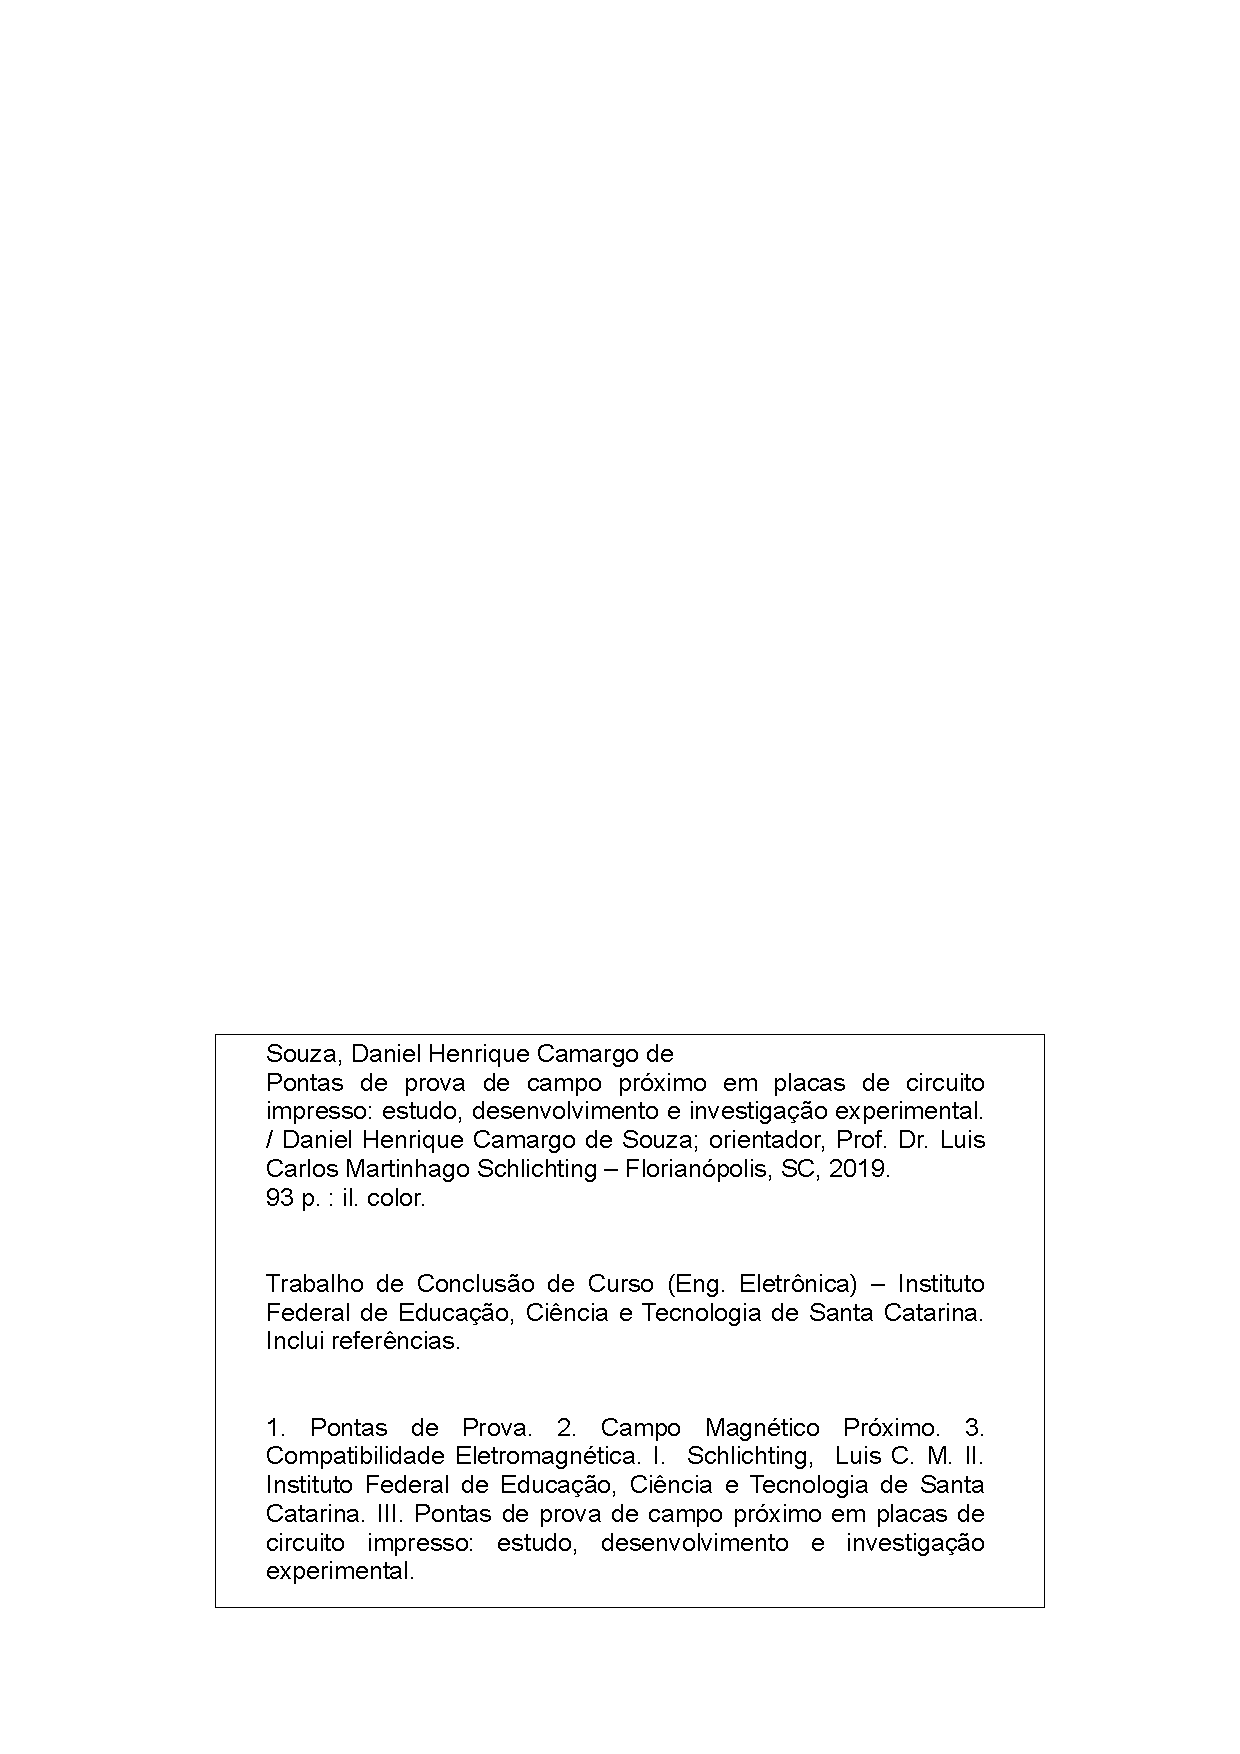
\includepdf{./pdf/fichacatalografica_final.pdf}     %Para Inclusão de modelo fornecido pela Biblioteca
\cleardoublepage

%\begin{fichacatalografica}
%    \sffamily
%    \vspace*{15cm}    % Posição vertical
%    \hrule    % Linha horizontal
%    
%    \begin{center}
%        % Minipage Centralizado
%        \begin{minipage}[c]{12.5cm} % Largura
%            \imprimirautor
%            \hspace{0.5cm} \imprimirtitulo / \imprimirautor. --
%            \imprimirlocal, \imprimirdata-
%            \hspace{0.5cm} \pageref{LastPage} p. : il.(alguma color.); 30 cm.%\\
%            \hspace{0.5cm} \imprimirorientadorRotulo \imprimirorientador\\
%            \hspace{0.5cm}
%            \parbox[t]{\textwidth}{\imprimirtipotrabalho~--~\imprimirinstituicao,
%            \imprimirdata.}\\
%            \hspace{0.5cm}
%            1. Palavra-chave1.
%            2. Palavra-chave2.
%            I. Orientador.
%            II. Universidade xxx.
%            III. Faculdade de xxx.
%            IV. Título\\
%            \hspace{8.75cm} CDU 02:141:005.7\\
%        \end{minipage}
%    \end{center}
%    \hrule
%\end{fichacatalografica}

% ----------------------------------------------------------
% ERRATA SEGUINDO NORMA TCC IFSC (OPCIONAL)
% ----------------------------------------------------------
%\begin{errata}
%    FERRIGNO, C. R. A. \textbf{Tratamento de neoplasias ósseas apendiculares com reimplantação de enxerto ósseo autólogo autoclavado associado ao plasma rico em plaquetas}: estudo crítico na cirurgia de preservação de membro em cães. 2011. 128 f. Tese (Livre-Docência) - Faculdade de Medicina
%    Veterinária e Zootecnia, Universidade de São Paulo, São Paulo, 2011.
%    \begin{table}[htb]
%        \center
%        \footnotesize
%        \begin{tabular}{|p{1.4cm}|p{1cm}|p{3cm}|p{3cm}|}
%            \hline
%            \textbf{Folha} & \textbf{Linha} & \textbf{Onde se lê} &
%            \textbf{Leia-se}\\
%            \hline
%            1 & 10 & auto-conclavo & autoconclavo\\
%            \hline
%        \end{tabular}
%    \end{table}
%\end{errata}
%
% ----------------------------------------------------------
% FOLHA APROVAÇÃO SEGUINDO NORMA TCC IFSC
% ----------------------------------------------------------
%\includepdf{folhadeaprovacao_final.pdf}     %Após as assinaturas é incluido digitalizado

\setcounter{page}{4}
\begin{folhadeaprovacao}
    \begin{center}
        \begin{center}
            \ABNTEXchapterfont\SingleSpacing\bfseries\Large\MakeUppercase\imprimirtitulo
        \end{center}
            
        \vspace*{2.0cm}
            
        \ABNTEXchapterfont\normalsize\bfseries\MakeUppercase\imprimirautor
            
        \vspace*{1.0cm}
    \end{center}
    
    
    \noindent\OnehalfSpacing Este Trabalho foi julgado adequado para obtenção do Título de Engenheiro Eletrônico em Outubro de 2020 e aprovado na sua forma final pela banca examinadora do Curso de Engenharia Eletrônica do instituto Federal de Educação Ciência, e Tecnologia de Santa Catarina.
        
    \vspace*{1.0cm}
    \begin{center}    
        \imprimirlocal, 26 de Outubro de 2020.
    \end{center}
    
    \noindent Banca Examinadora:
    
    \assinatura{Charles Borges de Lima, Dr. Eng.}
    \assinatura{Golberi de Salvador Ferreira, Dr. Eng.}
    \assinatura{Luis Martinhago Schlichting, Dr. Eng.}

\end{folhadeaprovacao}
\cleardoublepage

% ----------------------------------------------------------
% DEDICATORIA SEGUINDO NORMA TCC IFSC
% ----------------------------------------------------------
\begin{dedicatoria}

    \vspace*{\fill}
        Dedico este trabalho a minha Mãe, dona Jacira: Guerreira, correta e muito carinhosa, cuidou de mim e de minha irmã sozinha desde meus nove anos. Agradeço todos esses anos de luta, parceria e muito amor. Te amo muito Mãe e agradeço muito por poder te dizer isso todos os dias. Também dedico este trabalho ao meu Pai, seu Marco Aurélio: Muito carinhoso, trabalhador, querido por todos, sonhava em ver um dos seus filhos engenheiro. Isso antes que o câncer o levasse. Onde quer que estejas, eu te amo muito Pai.
    \vspace*{\fill}
    
\end{dedicatoria}


% ----------------------------------------------------------
% AGRADECIMENTOS SEGUINDO NORMA TCC IFSC
% ----------------------------------------------------------
\begin{agradecimentos}[AGRADECIMENTOS]
        Gostaria de agradecer primeiramente a minha família, mãe e irmã Jacira e Jéssica que sempre me deram apoio incondicional para que eu nunca desistisse de ser algo a mais. Gostaria de agradecer a minha companheira Isis, aos meus amigos de coração e a todos que de alguma forma participaram desse processo, seja com oportunidades únicas de aprendizado à um sorriso no rosto melhorando o dia-a-dia.
        
        Um agradecimento especial ao IFSC por proporcionar essa oportunidade de aprendizado contínuo com foco, persistência e sempre almejando uma sociedade melhor. Ao longo desses últimos 10 anos e com o trabalho de muita gente tornei-me finalmente técnico e engenheiro, e com meu trabalho poderei fazer da sociedade um lugar melhor.
        
        Outro agradecimento especial à Silicon Austria Labs por ter proporcionado essa oportunidade única de vida que foi fazer este projeto lá. Especialmente agradecido pelo carinho e cuidado que recebi de meus eternos amigos: Michael, Laura, Leonardo, Wolfgang, Aleš e Neža.

\end{agradecimentos}


% ----------------------------------------------------------
% EPIGRAFE SEGUINDO NORMA TCC IFSC
% ----------------------------------------------------------
%\begin{epigrafe}
%	
%    \noindent\textit{‘‘Não vos amoldeis às estruturas deste mundo, \\
%    mas transformai-vos pela renovação da mente, \\
%    a fim de distinguir qual éa vontade de Deus: \\
%    o que é bom, o que Lhe éagradável, o que éperfeito.\\
%    (Bíblia Sagrada, Romanos 12, 2)}
%    
%\end{epigrafe}

% ----------------------------------------------------------
% RESUMO SEGUINDO NORMA TCC IFSC
% ----------------------------------------------------------
% resumo na língua vernácula (obrigatório)
\setlength{\absparsep}{18pt} % ajusta o espaçamento dos parágrafos do resumo

\begin{resumo}

\noindent
\textbf{Palavras-chaves}: bobina de Helmholtz, campo magnético, indução magnética, sensor magnético. 

Na análise de transdutores é necessário um ambiente conhecido e controlado. No caso de transdutores magnéticos, esse ambiente é formado por um campo magnético conhecido, controlado e uniforme em toda a região de caracterização.

Para tal, é necessário um equipamento capaz de anular quaisquer fontes de campo magnético externo e, ainda sim, gerar um campo controlado e conhecido para a caracterização do transdutor na região de análise.

A bobina de Helmholtz é capaz de gerar no centro da sua estrutura uma indução magnética quase homogênea. Quanto maior a bobina e mais perto do centro da estrutura, maior a taxa de homogeneidade do campo produzido. Um conjunto de 3 bobinas em direções linearmente independentes é capaz de anular campos externos e também de gerar um campo homogêneo controlado por corrente.

Este trabalho trata do desenvolvimento de um equipamento com 3 bobinas de Helmholtz, eletronicamente controladas e conectadas a um computador, possibilitando o tratamento dos dados e geração de campos magnéticos de forma fácil e automática.

\end{resumo}

% ----------------------------------------------------------
% ABSTRACT SEGUINDO NORMA TCC IFSC
% ----------------------------------------------------------
\begin{resumo}[ABSTRACT]
\begin{otherlanguage*}{english}



\noindent
\textbf{Key-Words}: Helmholtz coil, magnetic field, magnetic induction, magnetic sensor. 


A known and controlled environment is required in the analysis of transducers. In the case of magnetic encoders, this environment is formed by a known, controlled and uniform magnetic field throughout the characterization region.

This requires an equipment capable of cancelling any external magnetic field sources and still generate a controlled and known field for the characterization of the transducer in the analysis region.

The Helmholtz coil is capable of generating in the center of its structure an almost homogeneous magnetic induction. The larger the coil and the closer to the center of the structure, the higher the homogeneity rate of the produced field. A set of 3 coils in linearly independent directions is able to annul external fields and also to generate a homogeneous field controlled by current.

This work deals with the development of an equipment with 3 Helmholtz coils, electronically controlled and connected to a computer, enabling the treatment of data and generation of magnetic fields easily and automatically.

\end{otherlanguage*}
\end{resumo}

% ----------------------------------------------------------
% LISTA DE ILUSTRAÇÕES
% ----------------------------------------------------------
\pdfbookmark[0]{\listfigurename}{lof}
\listoffigures*
\cleardoublepage

% ----------------------------------------------------------
% LISTA DE TABELAS
% ----------------------------------------------------------
\pdfbookmark[0]{\listtablename}{lot}
\listoftables*
\cleardoublepage

% ----------------------------------------------------------
% LISTA DE ABREVIATURAS E SIGLAS
% ----------------------------------------------------------
\begin{siglas}
   \item[IFSC] Instituto Federal de Educação Ciência e Tecnologia de Santa Catarina
   \item[SAL] \textit{Silicon Austria Labs} 
   \item[PCI] Placa de Circuito Impresso
   \item[CI] Circuito Integrado
   \item[MCU] Microcontrolador
   \item[USB] \textit{Universal Serial Bus}
   \item[RMS] \textit{Root Mean Square}
   \item[I2C] \textit{Inter-Integrated Circuit}
   \item[HAL] \textit{Hardware Abstraction Layer}
   \item[VISA] \textit{Virtual Instrument Software Architecture}
   \item[API] \textit{Application Programming Interface}
   \item[SMD] \textit{Surface Mount Device}
   \item[CC] Corrente contínua
   \item[CA] Corrente alternada
\end{siglas}

% ----------------------------------------------------------
% LISTA DE SIMBOLOS
% ----------------------------------------------------------
\begin{simbolos}
   \item[$T$] Tesla - Unidade de indução magnética
   \item[$mT$] Militesla - Unidade de indução magnética
   \item[$\mu T$] Microtesla - Unidade de indução magnética
   \item[$V$] Volts - Unidade de potencial elétrico
   \item[$mV$] Milivolts - Unidade de potencial elétrico
   \item[$A$] Ampere - Unidade de Corrente Elétrica
   \item[$mA$] Miliampere - Unidade de Corrente Elétrica
   \item[$\mu A$] Microampere - Unidade de Corrente Elétrica
   \item[$\Omega$] Ohms - Unidade de resistência elétrica
   \item[$H$] Henry - Unidade de indutância elétrica
   \item[$mH$] Henry - Unidade de indutância elétrica
   \item[$W$] Watts - Unidade de potência elétrica
   \item[$mW$] Miliwatts - Unidade de potência elétrica
   \item[$H_z$] Hertz - Unidade de Frequência 
   \item[$mm$] Milimetros - Unidade de comprimento 
   \item[$mm^{2}$] Milimetros Quadrados - Unidade de área
   \item[$mm^{3}$] Milimetros Cúbicos - Unidade de volume
\end{simbolos}

% ----------------------------------------------------------
% SUMÁRIO
% ----------------------------------------------------------
\pdfbookmark[0]{\contentsname}{toc}
\tableofcontents*
\cleardoublepage

% ----------------------------------------------------------
% ELEMENTOS TEXTUAIS
% ----------------------------------------------------------
\textual

% Cores para os códigos do MatLab
\definecolor{mygreen}{RGB}{28,172,0}    % color values Red, Green, Blue
\definecolor{mylilas}{RGB}{170,55,241}  % o lilas para códigos do MatLab

\lstset{language=Matlab,            %Que tipo de linguaguem os códigos serão
    %basicstyle=\color{red}, 		%normal fontsize
    %basicstyle=\ttfamily\footnotesize 	%fontsize small
    basicstyle=\ttfamily\scriptsize,		%fontsize verysmall
    %breaklines=false,%
    morekeywords={matlab2tikz},
    keywordstyle=\color{blue},%
    morekeywords=[2]{1}, keywordstyle=[2]{\color{black}},
    identifierstyle=\color{black},%
    stringstyle=\color{mylilas},
    commentstyle=\color{mygreen},%
    showstringspaces=false,%without this there will be a symbol in the places where there is a space
    numbers=left,%
    numberstyle={\tiny \color{black}},% size of the numbers
    numbersep=5pt, % this defines how far the numbers are from the text
    emph=[1]{for,end,break},emphstyle=[1]\color{red}, %some words to emphasise
    %emph=[2]{word1,word2}, emphstyle=[2]{style},    
}

% Elimina o Cabeçalho
\pagestyle{parpage}

%\part{Introdução}
\chapter{Introdução}

Para o desenvolvimento de um transdutor é necessária sua caracterização, ou seja, dadas excitações de natureza especifica, verificar a reação do transdutor a essas excitações. Assim, deve-se ter um ambiente de testes que forneça algum tipo de excitação conhecida, permitindo medidas precisas.

No caso de transdutores magnéticos, além da influência do meio (Permeabilidade magnética), há um campo terrestre que não é constante e que deve ser compensado.

Na empresa Silicon Austria Labs (SAL), onde foi feito este projeto, foi desenvolvido um transdutor magnético. Este transdutor necessitava ser caracterizado e para isso um equipamento que gerasse um campo magnético homogêneo e estático deveria ser construído.

Este trabalho descreve todo o projeto e construção deste equipamento que é baseado em bobinas de Helmholtz, uma bobina para cada direção do espaço (x, y, z), tendo como resultado uma bobina de Helmholtz 3D. O controle das bobinas e tratamento de dados também é desenvolvido nesse projeto.

\section{Objetivos}

\subsection{Objetivo geral}

O objetivo do projeto é desenvolver um equipamento que possa gerar um campo magnético homogêneo capaz de compensar o campo magnético da terra, sendo empregado para análise de sensores magnéticos. 
Os requisitos foram retirados da experiência do orientador do projeto com projetos anteriores de objetivo parecido. A seguir os requisitos para o campo magnético gerado pelas bobinas:    

\begin{itemize}
    \item Intensidade de indução magnética entre 1 $\mu$T e 1,25 mT em uma bobina principal, sendo as outras duas numa faixa de 1 $\mu$T e 0,25 mT
    \item Passo de indução de 1 $\mu$T ou menos.
    \item Diferença de intensidade de indução magnética de qualquer parte da região sob controle menor que 1\% da intensidade de campo no centro da região.
    \item Diferença do ângulo entre os vetores da região e o vetor central menor que um grau.
\end{itemize}

Todos esses requisitos devem ser cumpridos numa região grande o suficiente para o transdutor inteiro a ser caracterizado. No caso deste projeto, é definida uma região de 20 mm³, que é maior do que o transdutor desenvolvido pela SAL. O campo deve manter-se constante do começo ao fim de cada medida realizada.

\subsection{Objetivos específicos}

\begin{itemize}
    \item Projetar as bobinas de Helmholtz necessárias para gerar um campo tridimensional com o auxílio de um simulador.
    \item Projetar o suporte das bobinas de Helmholtz e todas as estruturas mecânicas relacionadas com o posicionamento dos dispositivos no sistema.
    \item Confeccionar as bobinas de Helmholtz e as peças do sistema.
    \item Projetar um sistema para controlar o campo gerado pelas bobinas de Helmholtz.
\end{itemize}

\chapter{Revisão teórica}



\section{Magnetismo}

Magnetismo é o fenômeno onde um material ou objeto causa uma força,
descrita como magnética, que repele ou atrai outros materiais e objetos susceptíveis. Este fenômeno é consequência de um movimento de cargas elétricas, algo que também surge em condutores elétricos de diversos tipos. Estas cargas em movimento são descritas em campos vetoriais, denominados campo magnético.\cite{callister2010}

A intensidade do campo pode ser representado pela letra H, onde sua unidade representa a intensidade do campo magnético, em $\frac{A}{m}$.\cite{callister2010}

A letra B representa a densidade de fluxo magnético, ou indução magnética, dado em T (Tesla). É uma relação do campo magnético com o meio. De forma simplificada na equação \ref{eq:bcalc} é apresentado o cálculo da indução magnética, onde µ representa a permeabilidade magnética do meio.\cite{callister2010}

\begin{equation}
    B =\mu H
    \label{eq:bcalc}
\end{equation}

\section{Campo Magnético Uniforme}
Campo Magnético é a região ao redor de um imã, na qual ocorre um efeito magnético. Esse efeito é percebido pela ação de uma Força Magnética de atração ou de repulsão. O campo magnético pode ser definido pela medida da força que o campo exerce sobre o movimento das partículas de carga, tal como um elétron.\cite{mussoi}

A representação visual do Campo Magnético é feita através de Linhas de Campo Magnético,
também conhecidas por Linhas de Indução Magnética ou ainda por Linhas de Fluxo Magnético, que são linhas envoltórias imaginárias. As linhas de campo magnético são linhas fechadas que saem do pólo norte e
entram no pólo sul. \cite{mussoi}

No caso de um imã em forma de ferradura, as linhas de campo entre as superfícies paralelas
dispõem-se praticamente paralelas, originando um campo magnético uniforme. No campo magnético
uniforme, todas as linhas de campo têm a mesma direção e sentido em qualquer ponto. A figura \ref{fig:muss2} mostra essa situação. \cite{mussoi}

\begin{figure}[H]
    \centering
     \caption{Linhas de campo uniforme e em imã permanente}
     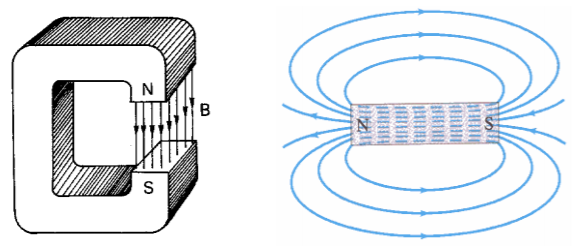
\includegraphics[width=0.8\textwidth]{./img/mussoi10.png}
     \caption*{Fonte: \cite{mussoi}}
     \label{fig:muss2}
\end{figure}


\section{Campo Magnético gerado no centro de uma Espira Circular}
Um condutor em forma de espira circular quando percorrido por corrente elétrica é capaz de
concentrar as linhas de campo magnético no interior da espira, como mostra a figura \ref{fig:campoc}. Isso significa que
a densidade de campo magnético resultante no interior da espira é maior que a produzida pela mesma
corrente no condutor retilíneo. \cite{mussoi} 

\begin{figure}[H]
    \centering
     \caption{Campo magnético em uma espira circular}
     \subfloat[Linhas de campo magnético mostradas através de pó de ferro]{%
       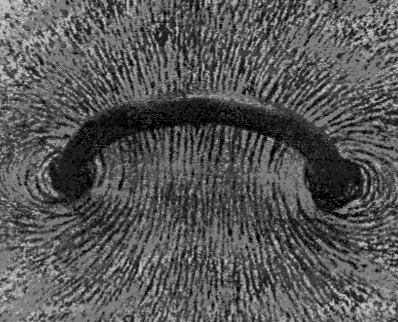
\includegraphics[width=0.45\textwidth]{./img/campoes.png}
     }
    % \hfill
     \subfloat[Esboço do campo vetorial magnético formado por uma espira]{%
      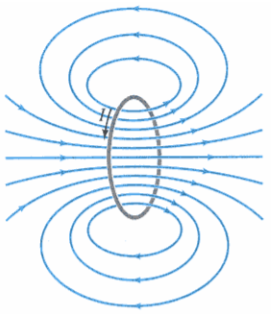
\includegraphics[width=0.33\textwidth]{./img/mussoi2.png}
     }
     \label{fig:campoc}
     \caption*{Fonte: \cite{mussoi}}
\end{figure}

\section{Bobina de Helmholtz}
Segundo \cite[p. 11, 12, tradução nossa]{caldeira2017}:

\begin{quoting}[rightmargin=0cm,leftmargin=4cm]
{\footnotesize 
Inventado por Hermann von Helmholtz em meados do século XIX, a bobina de Helmholtz é um dispositivo que produz campos magnéticos quase uniformes. É composto por duas bobinas circulares que são posicionadas paralelamente umas às outras a uma distância igual ao raio de cada uma e que partilham o mesmo eixo central (ver figura \ref{fig:bh}). Este dispositivo produz um campo magnético composto por linhas paralelas no centro do aparelho quando a corrente flui dentro dos fios que compõem a bobina. A direção do campo magnético pode ser previsto usando a regra da mão direita e a intensidade do campo magnético é calculada no centro usando uma derivação da lei Biot-Savart:

\begin{equation}
    B = 	\left ( \frac{4}{5} \right )^{\frac{3}{2}}\cdot \frac{\mu 0 \cdot n \cdot I}{R} [T]
    \label{eq:helmholtzCoil}
\end{equation}


}
\end{quoting}

Na equação \ref{eq:helmholtzCoil}, B representa a indução magnética, $\mu$0 a permeabilidade magnética do vácuo, n o número de espiras, I a corrente elétrica que passa pela bobina e R o raio dos enrolamentos da bobina e também a distância entre os dois enrolamentos que compõe a bobina de Helmholtz, isto pode ser observado na figura \ref{fig:bh}.

\begin{figure}[H]
    \centering
     \caption{Bobina de Helmholtz.}
     \subfloat[Geometria da bobina]{%
       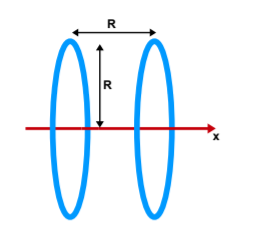
\includegraphics[width=0.3\textwidth]{./img/imagensExplicacoes/bobinaH.png}
     }
    % \hfill
     \subfloat[Esboço das linhas de campo]{%
      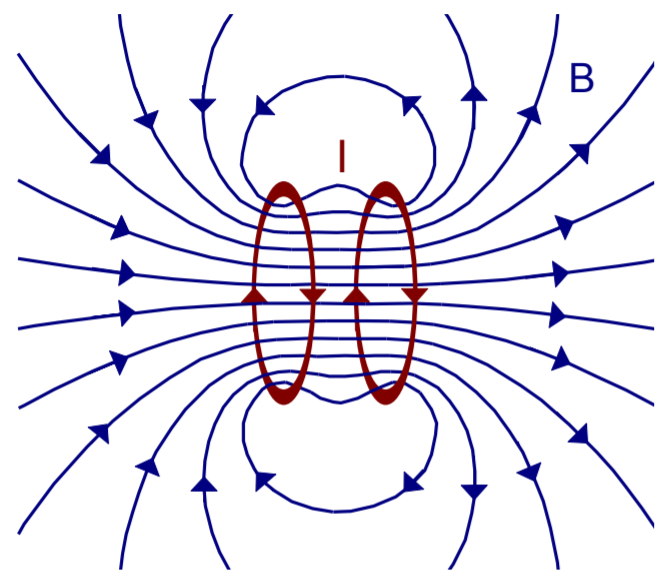
\includegraphics[width=0.3\textwidth]{./img/imagensExplicacoes/bobinaH2.png}
     }
     \label{fig:bh}
     \caption*{Fonte: \cite{caldeira2017}.}
\end{figure}

\subsection{Bobina de Helmholtz 3D}

Para um melhor entendimento do que seria uma bobina de Helmholtz 3D, na figura \ref{fig:bob3d} há uma ilustração de 3 bobinas de Helmholtz alinhadas de forma ortogonal, centradas no mesmo ponto, para gerar um campo homogêneo no centro da estrutura, cada par de enrolamentos paralelos é considerado uma bobina de Helmholtz e o conjunto dos 3 pares em direções ortogonais é a chamada bobina de Helmholtz 3D, que é capaz de gerar uma indução magnética em qualquer direção do espaço tridimensional, representado pela esfera no centro da estrutura.

\begin{figure}[H]
    \centering
     \caption{Ilustração das bobinas de Helmholtz.}
     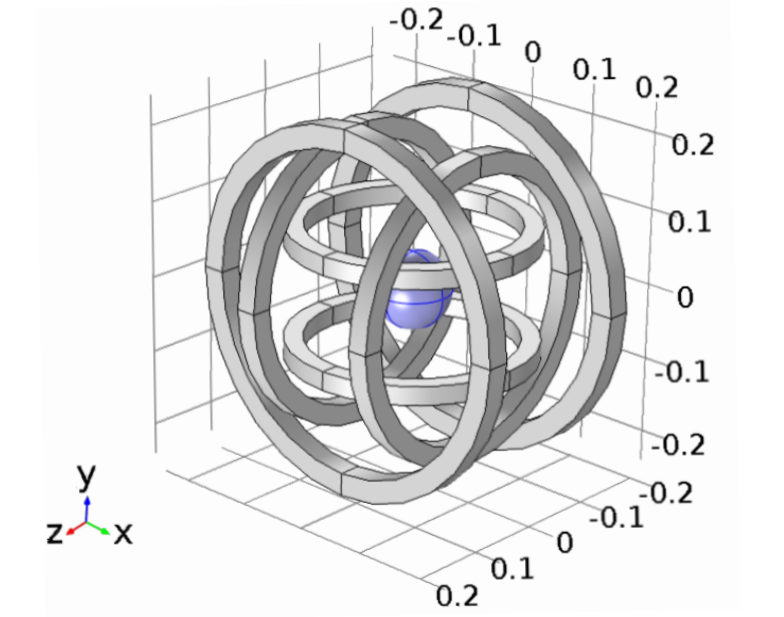
\includegraphics[width=0.65\textwidth]{./img/3dHMC.png}
     \caption*{Fonte: \cite{3dHelm}}
     \label{fig:bob3d}
\end{figure}

\section{Sensor magnético}

Um sensor magnético é um dispositivo capaz de detectar um campo magnético e transmitir as informações correspondentes. Um sensor magnético é, portanto,um transdutor que converte um campo magnético em informação. Por exemplo, uma agulha de bússola é um sensor magnético.\cite{popovic2003hall}

\section{Conversor de ponte completa (Ponte H)}
O conversor de ponte completa é um circuito utilizado para converter um sinal CC em um sinal CA, chaveando alternadamente entre as chaves S1 e S2 ou S3 e S4. Essa estrutura é também chamada de ponte H, se não houver chaveamento, pode-se apenas inverter a tensão da carga, assim como é demonstrado nas figuras \ref{fig:ponteh1} e \ref{fig:hart1} . \cite{hart2011power}

\begin{figure}[H]
    \centering
     \caption{Ponte H}
     \subfloat[Modelo do circuito]{%
       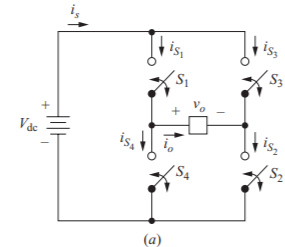
\includegraphics[width=0.5\textwidth]{./img/hart2.png}
     }
     \subfloat[Possibilidades de utilização]{%
       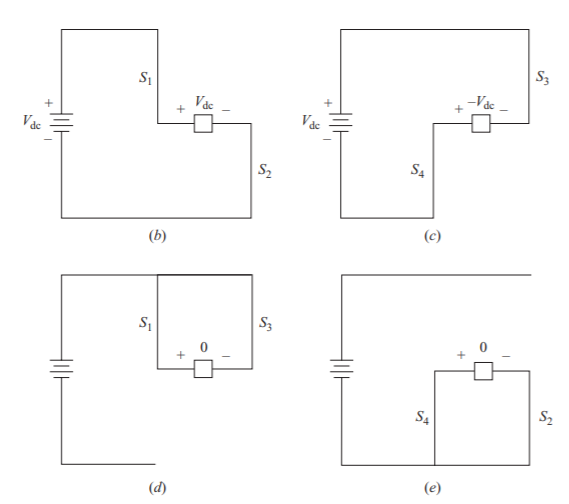
\includegraphics[width=0.5\textwidth]{./img/hart3.png}
     }
    % \hfill
     \caption*{Fonte:\cite{hart2011power}}\label{fig:ponteh1}
\end{figure}

\begin{figure}[H]
    \centering
     \caption{Estados da carga na ponte H}
     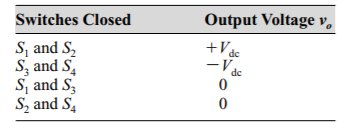
\includegraphics[width=0.65\textwidth]{./img/hart1.png}
     \caption*{Fonte: \cite{hart2011power}}
     \label{fig:hart1}
\end{figure}

Uma observação importante a comentar-se é que S1 e S4 não devem ser fechados ao mesmo tempo, nem S2 e S3 no caso da figura \ref{fig:ponteh1}. Caso contrário, existiria um curto-circuito através da fonte CC. \cite{hart2011power}

\section{Relação sinal ruído}

Um sinal, x(t), pode ser modelado como a soma do sinal desejado, s(t), e um sinal de ruído de faixa estreita, n(t), como mostrado na equação \ref{eq:sr}. \cite{haykinintrodução}

\begin{equation}
    \label{eq:sr}
    x(t) = s(t) + n(t)
\end{equation}

Os dois termos do lado direito da equação \ref{eq:sr} são aleatórios. O sinal é aleatório devido a imprevisibilidade de seu conteúdo de informação e o ruído é aleatório por natureza. Os dois parâmetros mais simples para descrever parcialmente uma variável aleatória são a média e a variância. Deslocamentos CC são considerados como sendo nulos. Consequentemente, para processos de média nula, uma simples medida da qualidade do sinal é a razão das variâncias dos sinais desejado e não desejado. Com esta base, a razão sinal/ruído é formalmente definida pela equação \ref{eq:sr2} \cite{haykinintrodução}

\begin{equation}
    \label{eq:sr2}
    SRN = \frac{E[s(t)^2]}{E[n(t)^2]}
\end{equation}

SRN é a relação sinal ruído e E é operador esperança. Para um sinal de comunicação, o nível do sinal quadrático é geralmente proporcional à potência. Consequentemente, a razão sinal/ruído é geralmente considerada como a relação da energia média do sinal por unidade de tempo pela energia média do ruído por unidade de tempo. \cite{haykinintrodução}
 
Segundo \cite{noiseRedArt}, para cada amostra de um sinal, se forem feitas N medidas, e a amostra for definida como a média dessas N medidas, a razão sinal ruído deste sinal é aumentada em $\sqrt{N}$. Isso é representado na equação \ref{eq:SRNn5}.

\begin{equation}
    \label{eq:SRNn5}
    SRN_N = \sqrt{N}\cdot SRN_1
\end{equation}

Neste caso a $SRN_1$ é representada pela razão entre o o sinal, s(kT), amostrado em períodos de tempo constante T e a variância do sinal $\sigma _n$ ou ruído RMS. Isso é mostrado na equação \ref{eq:as}. \cite{noiseRedArt}

\begin{equation}
    \label{eq:as}
    SRN_1 = \frac{s(kT)}{\sigma _n}
\end{equation}

\section{Python}
Nas palavras de \cite{bandeira2019}:
\begin{quoting}[rightmargin=0cm,leftmargin=4cm]
{\footnotesize 
Python é uma linguagem de programação de alto nível de abstração, utilizando o interpretador CPython como sua implementação padrão. Python é multiparadigma, encorajando o uso de programação orientada à objetos e de outros paradigmas para que o programador tenha a liberdade de decidir a maneira mais interessante de resolver diversos problemas. Introduzida em 1991 por Guido van Rossum,
Python possui uma gramática simples e poderosa.
}

\end{quoting}

\subsection{magPyLib}

É um pacote livre em Python para o cálculo de campos magnéticos, correntes e momentos magnéticos. Os campos magnéticos são determinados através de soluções analíticas as quais resultam em um tempo de computação muito mais rápido que soluções que empregam elementos finitos. \cite{magpy2020} 

\subsection{pySerial}

É uma biblioteca de código aberto que abstrai o acesso à porta COM virtual para o uso em computadores, empregado na programação \textit{python}, ou seja, da ao usuário o acesso a porta serial através de funções sem que o usuário tenha que se preocupar com o hardware da sua maquina. \cite{pySerial}

\subsection{pyVisa}

VISA é um acrônimo para \textit{Virtual Instrument Software Architecture}. VISA é uma API (\textit{Application Programming Interface}) de comunicação padrão da indústria de teste e medição para uso com dispositivos de teste e medição. Algumas vezes chamado de \textit{driver} de comunicação. VISA permite o desenvolvimento de programas independentemente do barramento de dados utilizado pelo instrumento. O uso de bibliotecas VISA permite a comunicação para muitas interfaces, como USB (\textit{Universal Serial Bus}) e Ethernet.\cite{visaRef}

A especificação VISA tem ligações explícitas com Visual Basic, C e G (linguagem gráfica do LabVIEW). Python pode ser usado para chamar funções de uma biblioteca compartilhada VISA (.dll, .so, .dylib) permitindo o desenvolvimento de diversas aplicações. Além disso, Python pode ser usado para acessar diretamente a maioria dos barramentos de dados usados por instrumentos, e é por isso que se pode prever a implementação do padrão VISA diretamente em Python. PyVISA é um \textit{wrapper} Python para bibliotecas compartilhadas VISA.\cite{pyvisaRef}

\chapter{Desenvolvimento do sistema}

O principal objetivo do projeto é o de controlar a indução magnética gerada em uma região especifica. A bobina de Helmholtz 3D é capaz de gerar um campo constante e homogêneo no centro de sua estrutura podendo ser controlada por corrente elétrica.

O digrama mostrado na figura \ref{fig:diag2} representa um sistema que utiliza diversas ferramentas para gerar as correntes na bobina de Helmholtz 3D. Um microcontrolador (MCU) verifica o campo gerado pelas bobinas através de um sensor magnético posicionado no centro das estruturas. O MCU se comunica com um computador, recebendo comando de controle das Pontes H que controlam as polaridades das correntes nas bobinas e também enviando os valores de campos lidos pelo sensor.

\begin{figure}[H]
    \centering
     \caption{Diagrama de blocos do sistema.}
     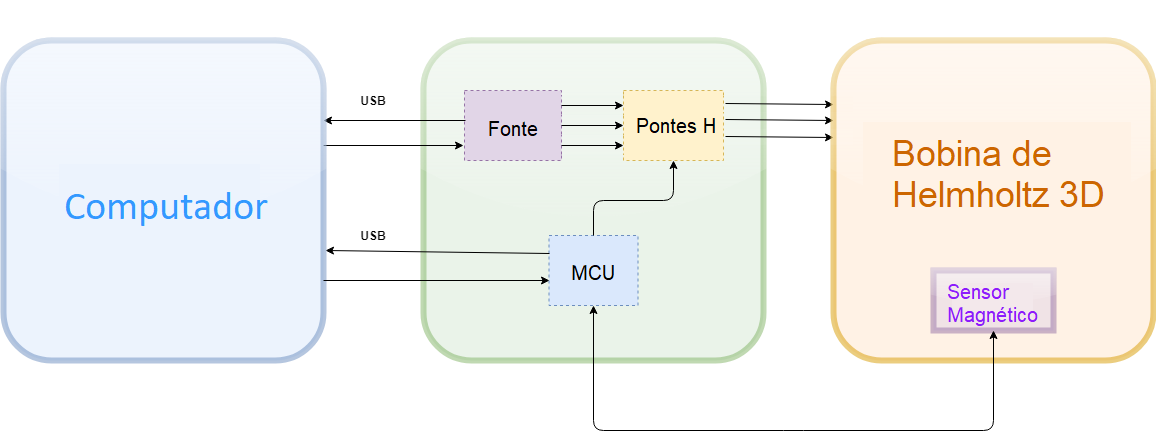
\includegraphics[width=1\textwidth]{./img/diagramas/Blocks diagram 2.png}
     \caption*{Fonte: Autor.}
     \label{fig:diag2}
\end{figure}

\section{Controle das bobinas}

\subsection{Fonte}

A fonte RIGOL 831-A \cite{RG831A} foi escolhida para a alimentação das bobinas de helmholtz. Contém 3 canais, um para cada bobina de Helmholtz a ser controlada, com o canal 3 de tensão negativa e referencia compartilhada com o canal 2. Segundo a folha de dados, a fonte tem resolução de corrente de 100 $\mu$A \cite{RG831A} e pode ser programada por VISA. Uma imagem ilustrativa pode ser vista na figura \ref{fig:font}.

\begin{figure}[H]
    \centering
     \caption{Fonte escolhida para o projeto.}
     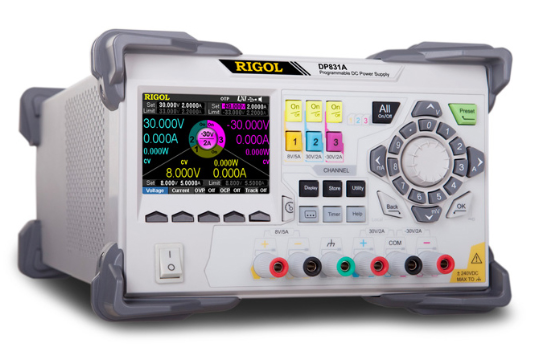
\includegraphics[width=0.8\textwidth]{./img/bob/fonte.png}
     \caption*{Fonte: Folha de dados Rigol DP831A.}
     \label{fig:font}
\end{figure}

\subsection{Ponte H}

Para este projeto foram necessárias 3 pontes H, uma para cada bobina Helmholtz que compõe a bobina de Helmholtz 3D. Ainda há a peculiaridade do canal com tensão negativa o qual a referencia está intrinsecamente conectada a outro canal positivo da fonte do projeto. Isso pode ocasionar um problema de detecção do sinal controle enviado pelo microcontrolador devido a referência da ponte H para o canal negativo estar conectada a uma tensão negativa e a do microcontrolador na referencia do circuito.

Para os canais positivos o CI (Circuito integrado) selecionado foi o DRV8838 \cite{drv8838}, esse é um CI  dedicado, que pode ser controlado com apenas 1 pino digital. A figura \ref{fig:pontHCI} ilustra um diagrama simplificado do DRV8838.

\begin{figure}[H]
    \centering
     \caption{Diagrama simplificado DRV8838.}
     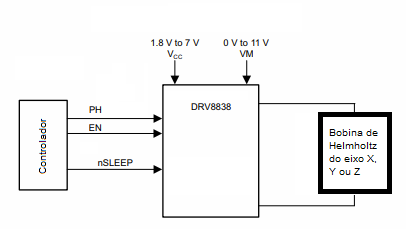
\includegraphics[width=0.8\textwidth]{./img/imagensExplicacoes/ponteHCI.png}
     \caption*{Fonte: Folha de dados DRV8838DSGR.\cite{drv8838}}
     \label{fig:pontHCI}
\end{figure}

Para garantir o funcionamento da ponte H no canal negativo optou-se por utilizar uma ponte H clássica \cite{ponteH} utilizando relés de estado sólido, que são transistores ativados por luz. Estes relés isolam eletricamente o MCU e a ponte H, fazendo com que o sinal de controle do microcontrolador seja detectado independente das referencias utilizadas no circuito da ponte H. Na figura \ref{fig:pontHOpt} é ilustrado o diagrama do componente utilizado para esse propósito.

\begin{figure}[H]
    \centering
     \caption{Diagrama do CPC1002N.}
     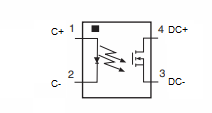
\includegraphics[width=0.5\textwidth]{./img/imagensExplicacoes/ponteHOpt.png}
     \caption*{Fonte: Folha de dados CPC1002N.}
     \label{fig:pontHOpt}
\end{figure}

No diagrama da figura \ref{fig:pontH} pode-se ver o esquemático da ponte H formada pela interligação desses relés, S1 e S4 funcionam juntos, assim como S2 e S3. Os dois conjuntos funcionam alternadamente, ou seja, se as chaves S1 e S4 foram ativadas, S2 e S3 serão desativadas, fazendo o sentido da corrente na carga circular da esquerda para a direita. Se as chaves S2 e S3 forem ativadas, S1 e S4 serão desativadas, fazendo com que a corrente na carga circule da direita para a esquerda.

\begin{figure}[H]
    \centering
     \caption{Ponte H isoladora.}
     \includegraphics[width=0.75\textwidth]{./img/imagensExplicacoes/ponte_h_rele.png}
     \caption*{Fonte: Autor.}
     \label{fig:pontH}
\end{figure}

A escolha dos componentes foi feita pela capacidade de corrente dos componentes que é maior que 500 mA. Essa é a corrente máxima escolhida para circular em cada bobina de Helmholtz e sera discutido na seção 3.3.

\subsection{Microcontrolador}

Era necessário que o microcontrolador tivesse um barramento I2C, 6 pinos de entrada/saída digital para o controle das pontes H e alguma forma de comunicação com o computador, sendo preferível a USB.

Com base nos parametros supracitados, o microcontrolador escolhido para o projeto foi o STM32L432, que emprega a arquitetura ARM Cortex-M4, com ponto flutuante em hardware. Dessa forma, empregou-se o kit de desenvolvimento STM32L432 KCU6. Na figura \ref{fig:diagArm} é apresentado um diagrama simplificado das funcionalidades do STM32L432 KCU6, enquanto que o kit pode ser observado na figura \ref{fig:kitArm}.

\begin{figure}[H]
    \centering
     \caption{Diagrama simplificado das funcionalidades do  STM32L432.}
     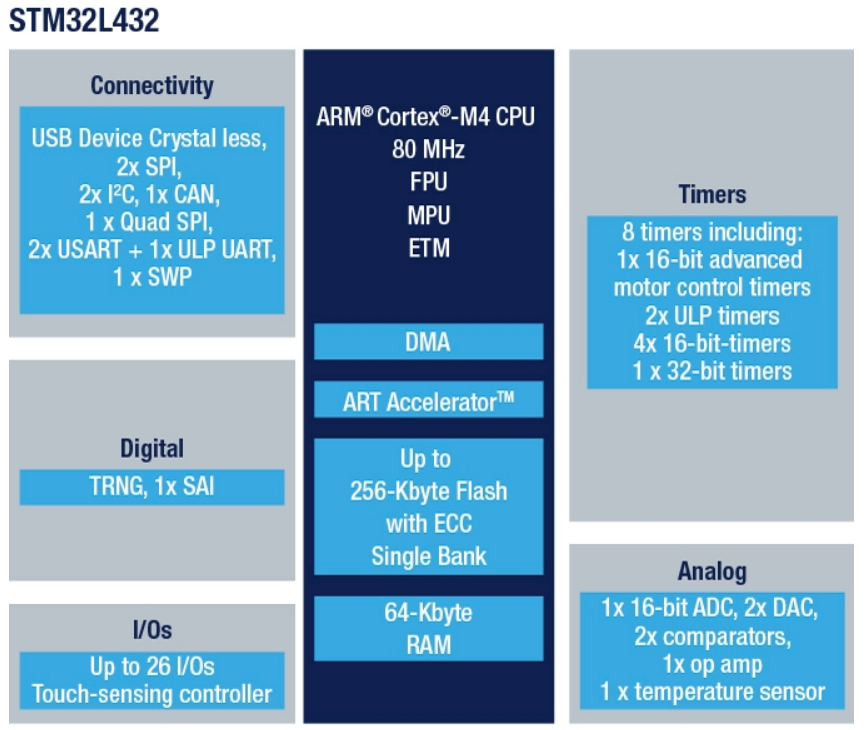
\includegraphics[width=0.8\textwidth]{./img/imagensExplicacoes/diagramaArm.png}
     \caption*{Fonte: ST.}
     \label{fig:diagArm}
\end{figure}


O kit foi escolhido por sua funcionalidade, preço, disponibilidade e facilidade de funcionamento. Todo o desenvolvimento do software necessário para a utilização do mesmo foi feito com o auxilio de uma ferramenta da empresa ST, o STM32Cube, que gera o código base para o funcionamento e configuração dos periféricos, e o TrueStudio - Atollic que é o editor de texto do programa, capaz de gravar e utilizar a depuração em hardware do kit.

O microcontrolador foi programado em C, utilizando bibliotecas HAL (Hardware Abstraction Layer) para facilitar e acelerar o desenvolvimento do firmware. As tarefas realizadas pelo microcontrolador foram implementadas na forma de uma máquina de estados que pode ser observada na figura \ref{fig:states}. As ações do microcontrolador dependem dos dados de comando recebidos serialmente. A tarefa de cada estado é explicada na tabela \ref{tab:states}.


\begin{figure}[H]
    \centering
     \caption{Kit de desenvolvimento STM32L432KCU6.}
     \includegraphics[width=0.4\textwidth]{./img/imagensExplicacoes/armkit.png}
     \caption*{Fonte: rs-online.}
     \label{fig:kitArm}
\end{figure}

\begin{table}[H]
    \centering
    \caption{Descrição dos estados.}
    \begin{tabular}{|p{4cm}|p{10cm}|}
     \hline
     \textbf{Simbolo do estado} & \textbf{Descrição do estado} \\
     \hline
     IDDLE & Estado que aguarda o recebimento de outro estado. \\ \hline
     I &  Define a polaridade para \textit{set} na ponte H conectada ao canal 2 e envia de volta `` `I' done!". \\ \hline
     i & Define a polaridade para \textit{set} na ponte H conectada ao canal 2 e envia de volta `` `i' done!". \\ \hline
     M & Define a polaridade para \textit{set} na ponte H conectada ao canal 3 e envia de volta `` `m' done!". \\ \hline
     m & Define a polaridade para \textit{set} na ponte H conectada ao canal 3 e envia de volta `` `M' done!". \\ \hline
     E & Define a polaridade para \textit{set} na ponte H conectada ao canal 1 e envia de volta `` `E' done!". \\ \hline
     e & Define a polaridade para \textit{set} na ponte H conectada ao canal 1 e envia de volta `` `e' done!". \\ \hline
     S & Coloca todas as polaridades em uma referência e envie de volta `` `S' done!". \\ \hline
     C & Executa procedimentos de medição contínuos e envie-os para a comunicação USB sem voltar ao estado IDDLE.\\ \hline 
     D & Executa apenas um procedimento de medição e envia o resultado dos dados para a comunicação pela USB retornando as estado IDDLE.\\ \hline
     
    \end{tabular}
    \label{tab:states}
\end{table}

As polaridades mencionadas na tabela \ref{tab:states}, \textit{set} e \textit{reset}, são nomes dados a polaridades opostas, ou seja, se \textit{set} for representado por estado lógico alto, \textit{reset} é representado pelo estado lógico baixo. Há um estado diferente para cada polaridade possível nas bobinas de Helmholtz. Além do estado S, utilizado para calibração e do estado C, utilizado no desenvolvimento das bobinas, há também um estado D, utilizado para requisitar, adquirir e processar as informações da indução magnética provenientes do sensor MMC3416 (Sensor que se comunica por protocolo I2C, seção 3.1.4). Dentro desse estado, o microcontrolador adquire os dados dos registradores do sensor, logo após tratamento, os envia para o computador.

A espera por comandos no estado IDDLE é realizada através de \textit{pooling}, que é um laço em software que espera por um evento, verificando constantemente o \textit{buffer} de entrada serial do microcontrolador para troca de estado.

\begin{figure}[H]
    \centering
     \caption{Diagrama da maquina de estados implementada no STM32L432KCU6.}
     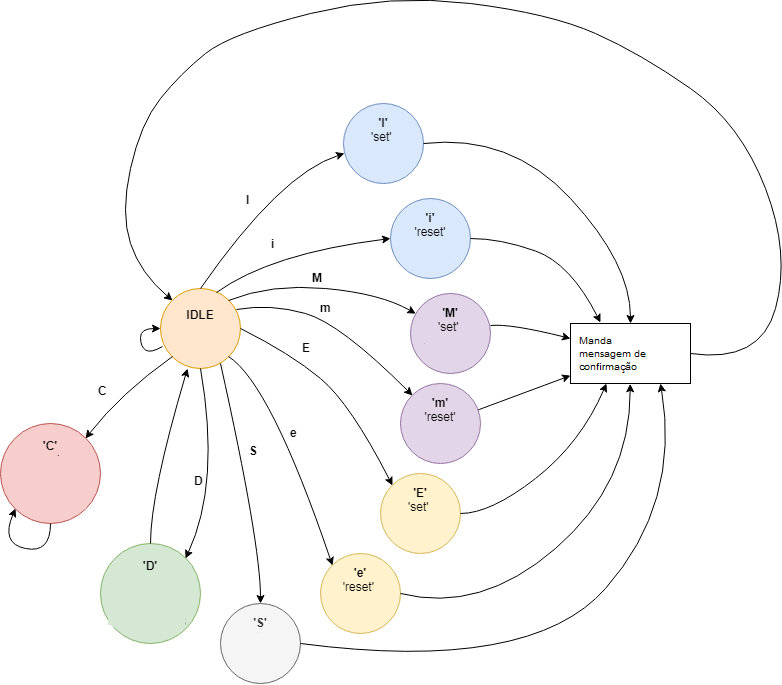
\includegraphics[width=0.8\textwidth]{./img/imagensExplicacoes/stateMachine.png}
     \caption*{Fonte: Autor.}
     \label{fig:states}
\end{figure}

\subsection{Sensor magnético}

O MMC3416 \cite{mcc3416} foi selecionado devido suas características de escala e resolução, mede em 3 direções, permitindo o ajuste de \textit{offset} pela utilização de uma função de \textit{set-reset} que anula o offset da medição \cite{AN213Ref}. É alimentado entre 1,8 e 3,6V e se comunica através do barramento I2C. Na figura \ref{fig:sensDiag} é apresentado o diagrama interno do componente.

\begin{figure}[H]
    \centering
     \caption{Diagrama interno do sensor.}
     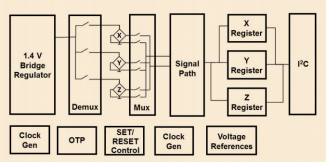
\includegraphics[width=0.8\textwidth]{./img/imagensExplicacoes/sensorDiag.png}
     \caption*{Fonte: Folha de dados do MMC3416.}
     \label{fig:sensDiag}
\end{figure}

A maior resolução possivelmente utilizada para este projeto seria de 1 $\mu$T. O MMC3416 tem resolução de 0.05 $\mu$T até 0.2 $\mu$T por \textit{bit} menos significativo, tendo uma escala com tamanho de 16 bits. Esse CI mede uma escala de $\pm$1600 $\mu$T, sendo este valor absolutamente maior que 1250 $\mu$T (Requisitos de geração da bobina). Além disso, o ruído \textit{RMS} (Ruído da raiz quadrada média) máximo é cerca de 0.15 $\mu$T, o que não acarreta erros significativos na medição.

Para rapidez no desenvolvimento empregou-se uma placa de avaliação na qual o sensor já vem montado. Essa placa é apresentada na figura \ref{fig:sensEval} e a mesma foi utilizada para o desenvolvimento do projeto.

\begin{figure}[H]
    \centering
     \caption{Hardware da placa de avaliação do sensor.}
     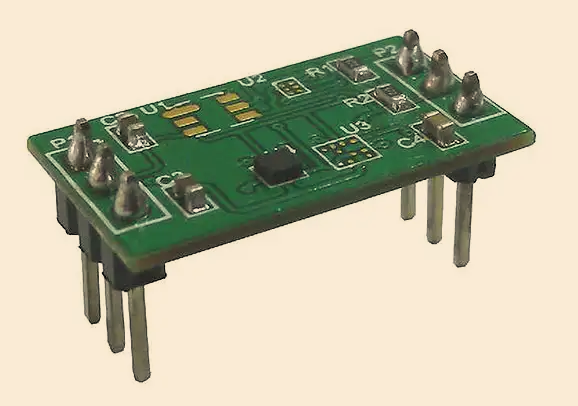
\includegraphics[width=0.6\textwidth]{./img/imagensExplicacoes/sensorEval.png}
     \caption*{Fonte: Folha de dados da placa de avaliação.}
     \label{fig:sensEval}
\end{figure}

\section{Placas de Circuito Impresso}

Mesmo utilizando uma placa de avaliação e um kit microcontrolado, era necessária a interligação entre essas placas em um único sistema. Assim, foram projetadas duas PCIs (Placas de Circuito Impresso)  empregando o software EAGLE (7.1) \cite{EagleWiki}. Uma PCI para receber o cabeamento necessário para o sensor e a outra, para conexão do kit microcontrolado com as demais partes do sistema. 

\subsection{PCI do sensor}

É a PCI mais simples, o sensor é centrado exatamente no meio da placa. Na figura \ref{fig:esqDesSens} é mostrado o esquemático e projeto do circuito. O circuito é uma simples ligação dos pinos do sensor até um conector do tipo KK \cite{KKcon}. Cada pino de sinal é acompanhado por um pino de referencia, sendo o cabo formado por pares levemente trançados para diminuir possíveis interferências no sinal.

\begin{figure}[H]
    \centering
     \caption{PCI do sensor}
     \subfloat[Esquemático]{%
       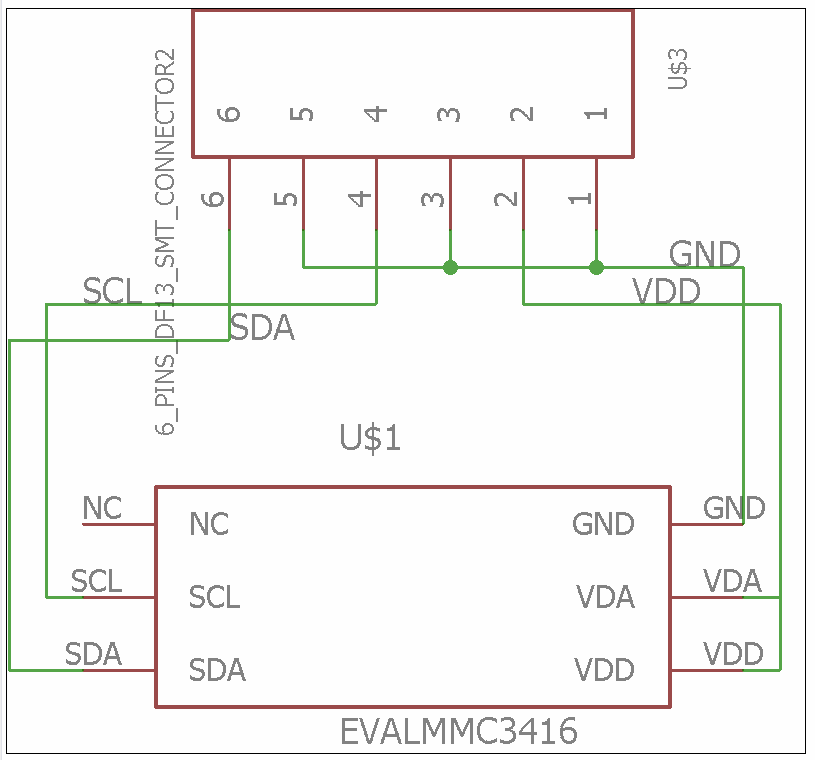
\includegraphics[width=0.35\textwidth]{./img/PCBs/esquematicoSensor.png}
     }
     \subfloat[Desenho de PCI]{%
       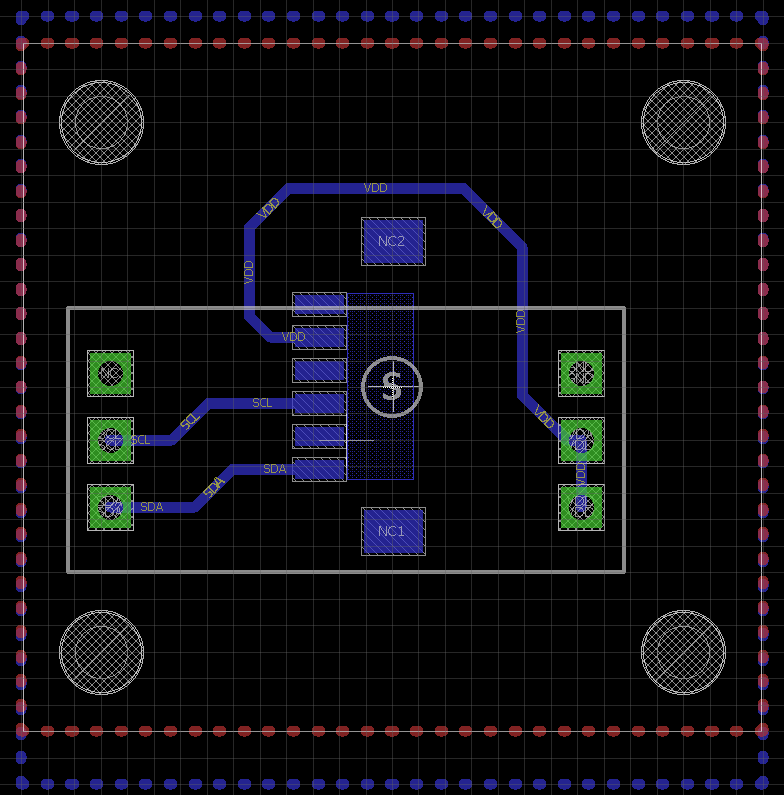
\includegraphics[width=0.35\textwidth]{./img/PCBs/desenhoSensor.png}
     }
    % \hfill
     \caption*{Fonte: Autor.}\label{fig:esqDesSens}
\end{figure}


\subsection{PCI do sistema}

A PCI do sistema une as bobinas de Helmholtz, o sensor, a fonte e o computador. Estão nela inseridos as pontes H, conectores para as bobinas, para o sensor e para a fonte. Também, permite o encaixe do kit STM32, que é conectado ao computador através do um cabo USB. A figura \ref{fig:esqMain} apresenta o esquemático dessa PCI.

\begin{figure}[H]
    \centering
     \caption{Esquemático da placa principal}
     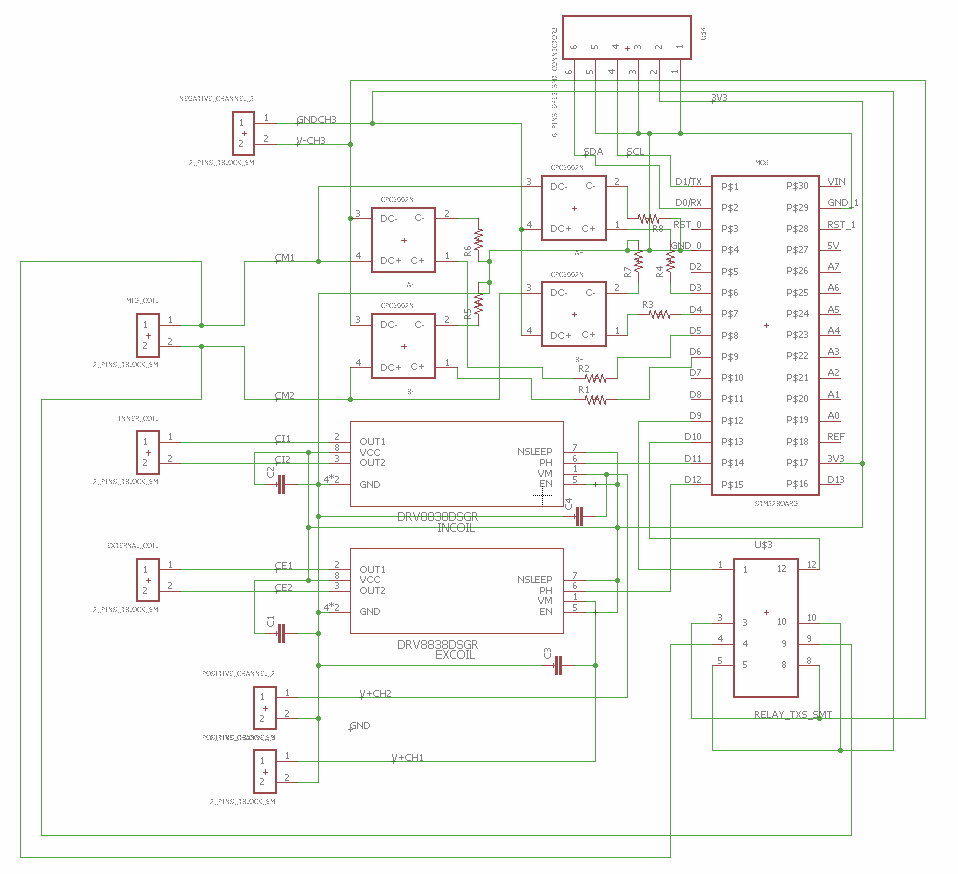
\includegraphics[width=1\textwidth]{./img/PCBs/esquematicoMain.png}
     \caption*{Fonte: Autor.}\label{fig:esqMain}
\end{figure}

No projeto da placa pode-se observar alguns furos metalizados (figura \ref{fig:desMain}), tendo trilhas tanto na parte superior quanto na inferior da PCI. Todos os componentes referentes às pontes H são SMDs. Na figura \ref{fig:pbcMain} é apresentado a PCI montada, todos os componentes foram inseridos manualmente, com colocação de pasta de solda utilizando um \textit{stencil}. Para a solda foi utilizado um forno elétrico doméstico.

\begin{figure}[H]
    \centering
     \caption{Desenho da PCI principal}
     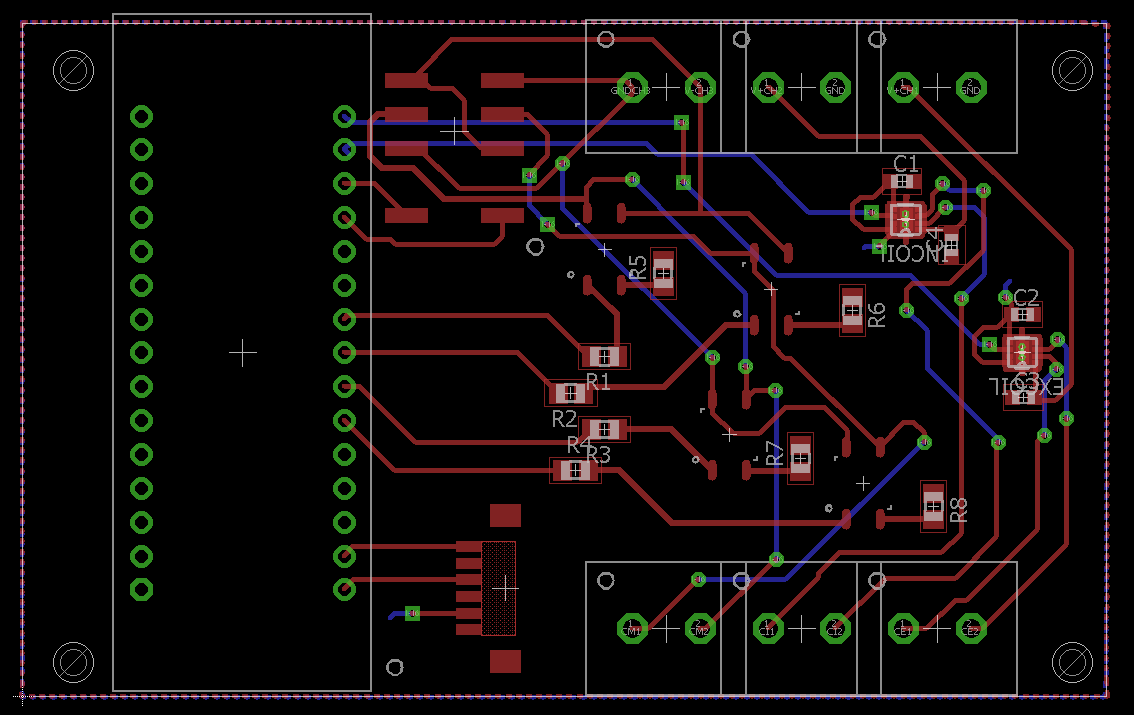
\includegraphics[width=0.55\textwidth]{./img/PCBs/desenhoMain.png}
     \caption*{Fonte: Autor.}\label{fig:desMain}
\end{figure}

\section{Bobinas de Helmholtz}

Para o auxílio no projeto das bobinas, tal como estimativa de formato e intensidade do campo, um simulador foi desenvolvido utilizando a magpylib \cite{magpy2020}.

Analisando-se os tamanhos de fios disponíveis, decidiu-se trabalhar com o AWG 23, utilizando a máxima corrente de 500 $mA$. Este valor de corrente não gerará potências maiores que 2 $W$, importante para o não derretimento das estruturas mecânicas de suporte das bobinas. Esse valor de corrente foi decidido após algumas iterações utilizando o simulador descrito na seção seguinte (3.3.1), através da resistência estimada das bobinas.

\subsection{Simulador}

Para simular as espiras nas posições corretas é necessário um modelo em função da geometria das bobinas de Helmholtz. Na modelagem, foi utilizada a secção de corte transversal dos enrolamentos, como mostrado na figura \ref{fig:cross}.

\begin{figure}[H]
    \centering
     \caption{Exemplo de seção transversal da bobina.}
     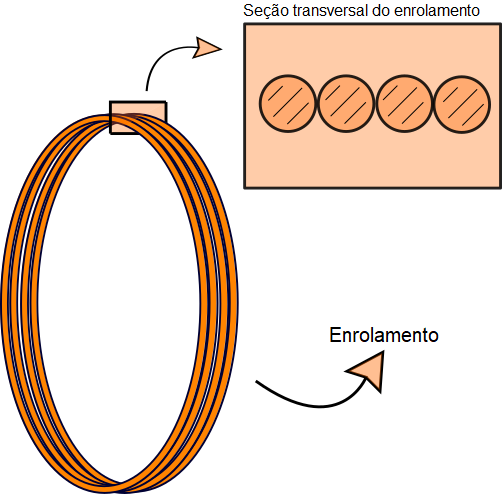
\includegraphics[width=0.5\textwidth]{./img/imagensExplicacoes/coil explanation.png}
     
     \caption*{Fonte: Autor.}\label{fig:cross}
\end{figure}

Os parâmetros para a modelagem da bobina estão sendo mostrados na figura \ref{fig:model}.

\begin{figure}[H]
    \centering
     \caption{Modelagem das bobinas}
     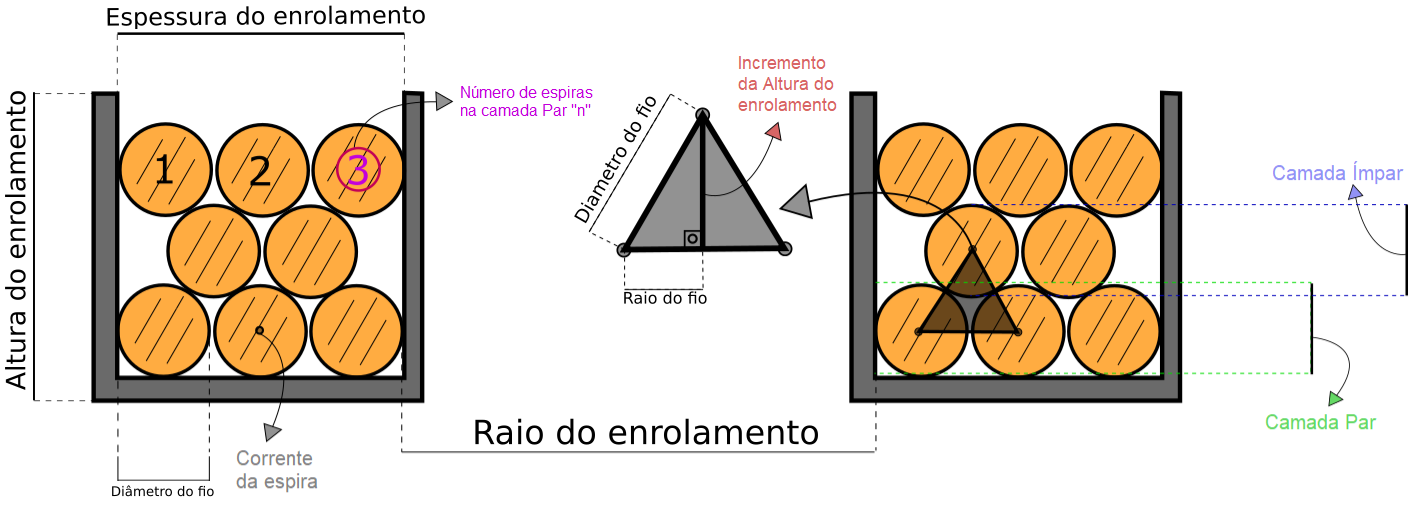
\includegraphics[width=1.05\textwidth]{./img/imagensExplicacoes/coil cross cut.png}
     
     \caption*{Fonte: Autor.}\label{fig:model}
\end{figure}

A partir do modelo das bobinas fez-se um programa em \textit{python} utilizando a \textit{magpylib}, capaz de calcular iterativamente o raio necessário para cada bobina, de forma a obter-se o campo desejado na região de interesse.

Além dos parâmetros do modelo, haviam outros parâmetros de entrada necessários para as iterações:

\begin{itemize}
    \item Número de laços nas camadas de laços Par.
    \item Número de camadas de laços Par e Ímpar.
    \item A indução desejada com a corrente máxima da bobina em $mT$.
    \item Corrente máxima da bobina em $mA$.
\end{itemize}

O modelo utiliza os parâmetros supracitados garantindo o funcionamento das bobinas da maneira esperada. Para facilitar a construção, ao invés do software utilizar o número de espiras de cada enrolamento, ele utiliza com o número de camadas pares e ímpares como parâmetro de entrada. No código a seguir é ilustrado o uso desses parâmetros para o cômputo do raio correto das bobinas.

%% Codigo
\inputminted[
frame=lines,
framesep=1mm,
baselinestretch=0.5,
fontsize=\footnotesize,
linenos
]{python}{codigos/sim.py}

O programa gera vários gráficos da geometria das bobinas e estima valores sobre parâmetros, tais como, comprimento de fio e potência dissipada.

Nos gráficos da figura \ref{fig:eixos} são mostrados o formato das 3 bobinas de Helmholtz em seus respectivos eixos. A bobina z tem mais enrolamentos que as outras pelo fato de ter uma especificação de campo maior. O que é visível nesses gráficos é que cada bobina foi dimensionada de forma ortogonal umas as outras, gerando 3 campos magnéticos em 3 direções linearmente independentes.

\begin{figure}[H]
    \centering
     \caption{Ilustração gráfica das bobinas}
     \subfloat[eixo 'z']{%
       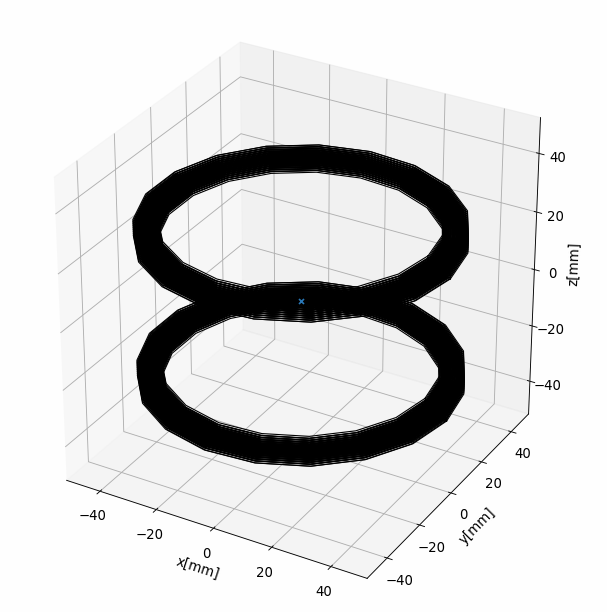
\includegraphics[width=0.3\textwidth]{./img/simulacao/zcoil.png}
     }
     \subfloat[eixo 'y']{%
       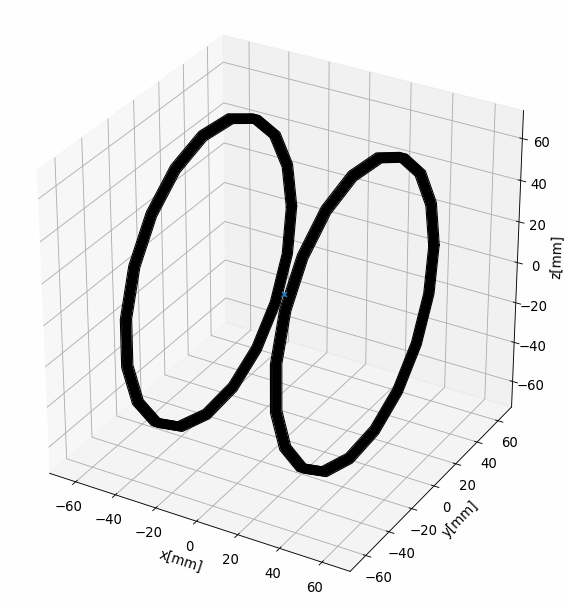
\includegraphics[width=0.3\textwidth]{./img/simulacao/ycoil.png}
     }
     \subfloat[eixo 'x']{%
       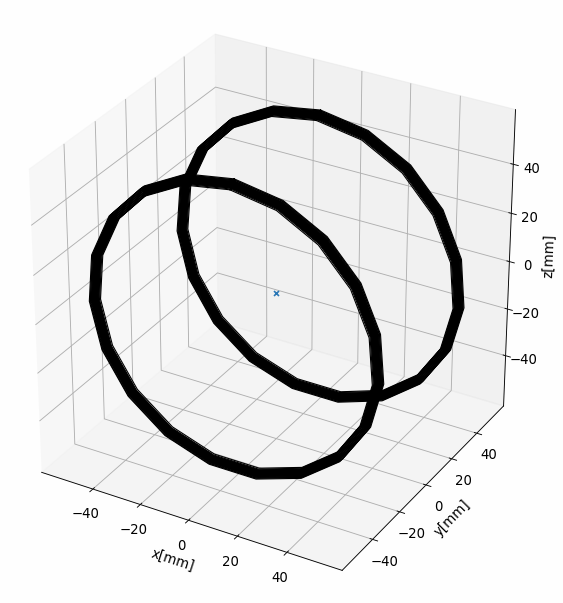
\includegraphics[width=0.3\textwidth]{./img/simulacao/xcoil.png}
     }
    % \hfill
     \caption*{Fonte: Autor.}\label{fig:eixos}
\end{figure}

Concomitante aos gráficos da figura \ref{fig:eixos}, são mostrados gráficos do campo magnético gerado na região de interesse. As figuras \ref{fig:grafz}, \ref{fig:grafy} e \ref{fig:grafx} demonstram curvas de nível em um plano de 20 mm x 20 mm no centro de cada uma das três estrutura. Exitem 4 gráficos em cada uma das 3 figuras supracitadas. Todos os 4 tem unidades de mm nos eixos horizontal e vertical. Em cada gráfico aparecem curvas de nível com seus respectivos valores, sendo as cores do gráfico uma ideia de potencial.

O gráfico superior esquerdo representa valores percentuais. Cada valor do gráfico é a diferença percentual de indução magnética do ponto em relação a indução magnética no centro da estrutura (0,0).

Nos demais gráficos, os valores das curvas de nível representam valores da indução magnética absoluta, todos dados em $\mu$T. O que difere os 3 gráficos é a direção vetorial do campo, sendo todos os pontos do gráfico superior direito na direção x, o inferior esquerdo na direção y e o inferior direito na direção z.

Os gráficos da figura \ref{fig:grafz} são relacionado com a bobina da figura \ref{fig:eixos} (a), sendo os gráficos das figuras \ref{fig:grafy} e \ref{fig:grafx} relacionados à figura \ref{fig:eixos} (b) e (c) respectivamente.
    
\begin{figure}[H]
    \centering
     \caption{Gráfico da indução magnética estimada na região de interesse (z)}
     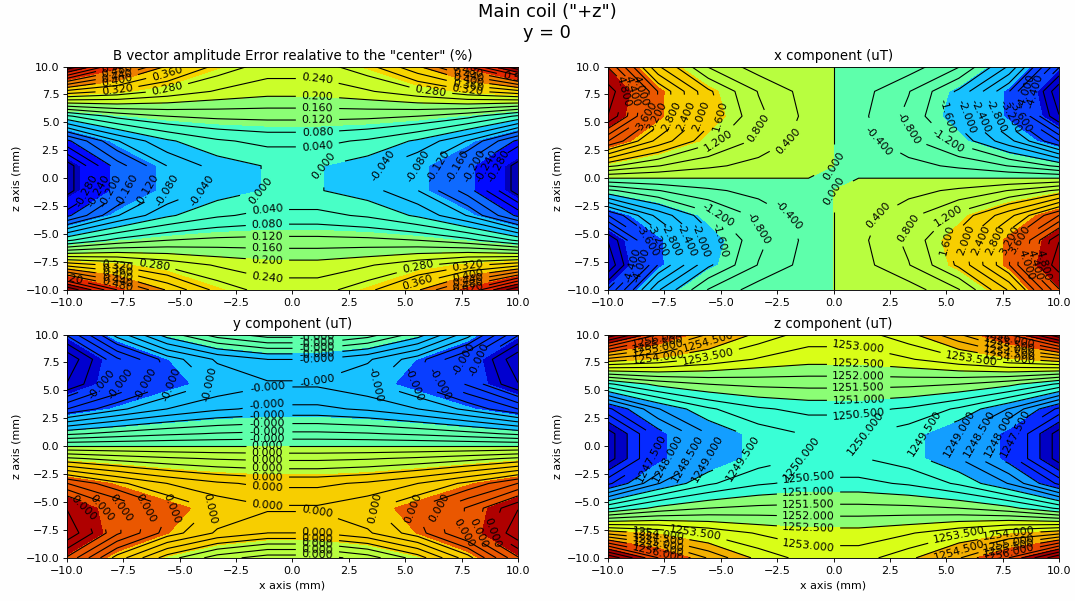
\includegraphics[width=1\textwidth]{./img/simulacao/mainCoilZ.png}
     \caption*{Fonte: Autor.}\label{fig:grafz}
\end{figure}


\begin{figure}[H]
    \centering
     \caption{Gráfico da indução magnética estimada na região de interesse (y)}
     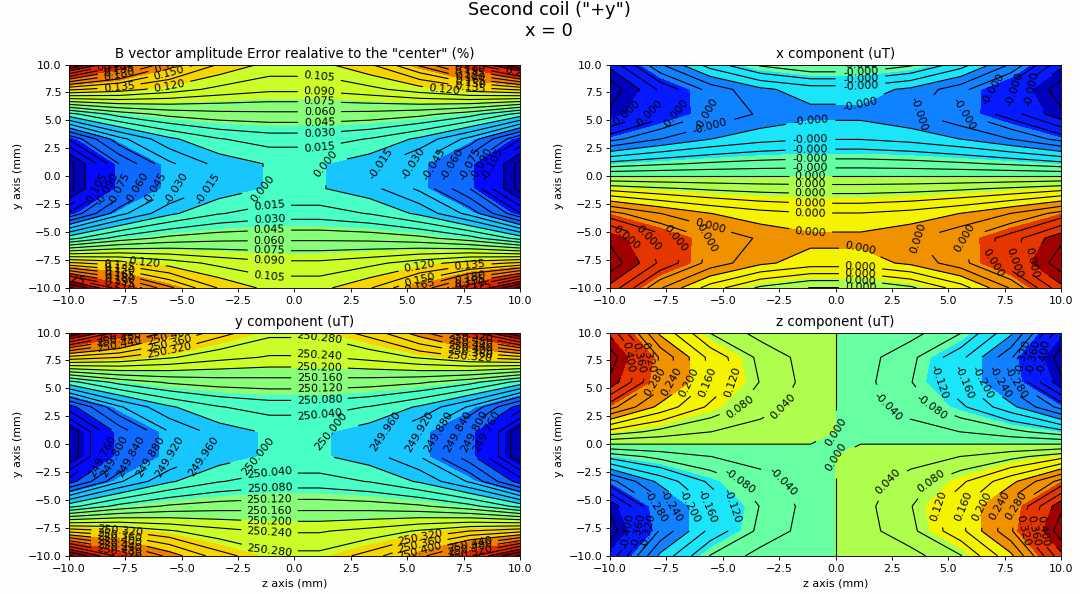
\includegraphics[width=1\textwidth]{./img/simulacao/secondCoily.png}
     \caption*{Fonte: Autor.}\label{fig:grafy}
\end{figure}

\begin{figure}[H]
    \centering
     \caption{Gráfico da indução magnética estimada na região de interesse (x)}
     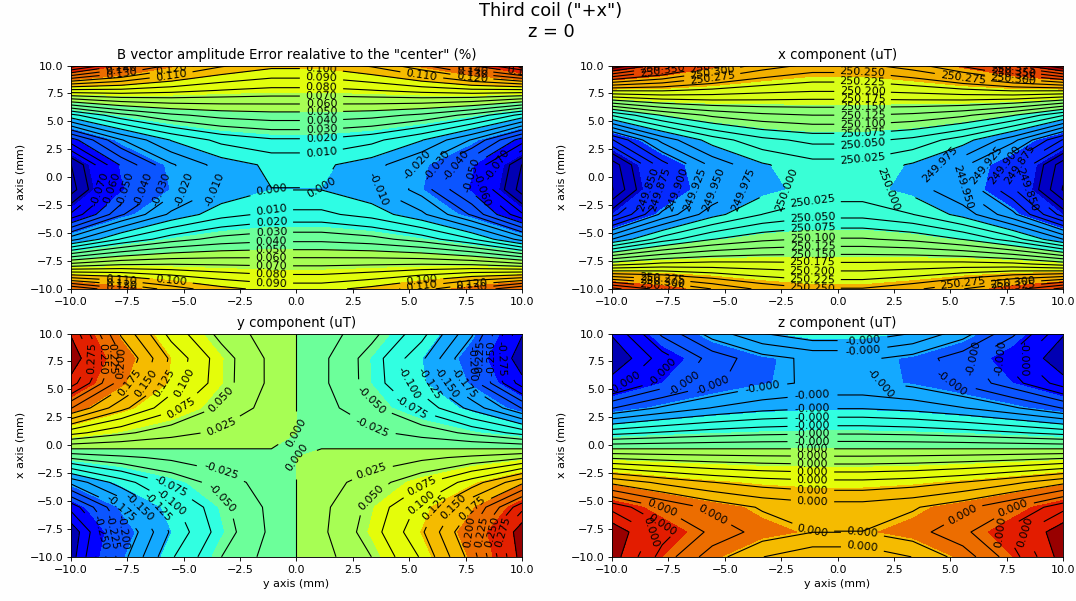
\includegraphics[width=1\textwidth]{./img/simulacao/thirdCoilx.png}
     \caption*{Fonte: Autor.}\label{fig:grafx}
\end{figure}

Há dois parâmetros a serem analisados com as figuras \ref{fig:grafz}, \ref{fig:grafy} e \ref{fig:grafx}: 

\begin{itemize}
    \item A diferença de intensidade da indução magnética gerada em cada ponto da região de interesse em relação a intensidade gerada no centro da bobina (0,0).
    \item A diferença de direção do campo gerado em cada ponto do gráfico em relação a direção do ponto central do gráfico.
\end{itemize}

Para notar a diferença de intensidade da indução magnética, basta observar o gráfico superior esquerdo das figuras anteriores. Se não houver nenhum valor maior que 1,  significa que em questão de módulo, a bobina cumpre com o requisito de homogeneidade de amplitude segundo objetivos. Para o cumprimento do requisito de direção de campo, o ângulo formado pelos vetores em cada ponto do gráfico não deve ser maior do que um grau em relação à direção de interesse de cada bobina.

Na verificação dessa diferença de direção é necessária a análise do ângulo formado em cada ponto do vetor em relação a direção desejada. Ou seja, na bobina com direção desejada em z, é necessária a análise do ângulo formado nos planos zy e zx. Se os ângulos dos vetores em relação a direção z forem menores do que um grau nos dois planos, então o requisito de homogeneidade de direção é cumprido.

Para a análise foram verificados nos gráficos os pontos de maiores amplitudes nos dois planos e na direção desejada. Nessa análise é realizado o cálculo da tangente do vetor utilizando o cateto oposto (outra direção) e o cateto adjacente (direção de interesse). O resultado do cálculo é comparado com a tangente de um grau. Se for menor, a bobina Helmholtz passa no teste e a região de interesse é considerada homogênea. Na equação \ref{eq:anghomo} é possível observar a relação entre a tangente de um grau e a tangente do vetor a ser analisado.

\begin{equation}
    \hspace{2pt}\textrm{tg}(1º) = 0.01745 \geq \frac{vetor_{outraDirecao}}{vetor_{DirecaoDeInteresse}}
    \label{eq:anghomo}
\end{equation}

O valor das tangentes nos dois planos, para o ponto com maior amplitude nas direções não desejadas em cada bobina Helmholtz é apresentado na figura \ref{fig:raz}. Pode-se observar que os valores encontrados foram até 5 vezes menores que o valor da tangente de um grau, validando o requisito de ângulo dos vetores na região de interesse segundo objetivos.

\begin{figure}[H]
    \centering
     \caption{Razões entre a direção não desejada e a direção desejada (código em python)}
     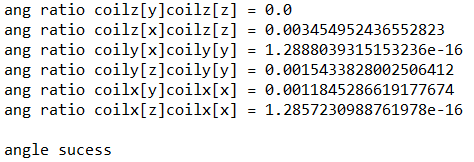
\includegraphics[width=0.8\textwidth]{./img/simulacao/angulo_console.png}
     \caption*{Fonte: Autor.}\label{fig:raz}
\end{figure}

Na figura \ref{fig:3dcoil} é possível observar que há espaço entre as bobinas, não havendo sobreposição de um enrolamento em outro, ou seja, quando a bobina for confeccionada, os enrolamentos terão distância radial suficiente para não colidirem fisicamente na hora que forem enrolados.

\begin{figure}[H]
    \centering
     \caption{Ilustração das 3 bobinas.}
     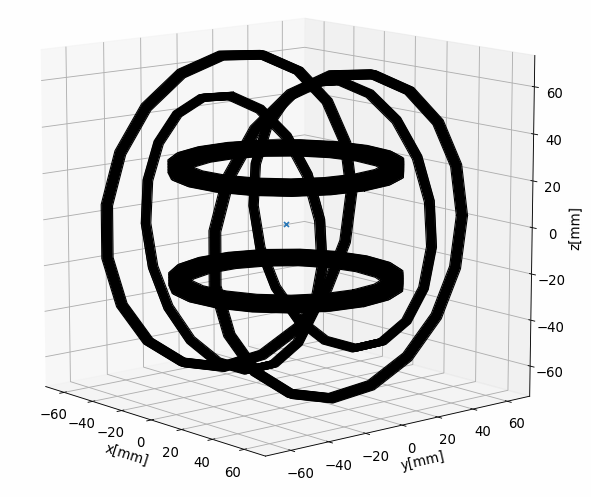
\includegraphics[width=0.65\textwidth]{./img/simulacao/desenhoCoil3D.png}
     \caption*{Fonte: Autor.}\label{fig:3dcoil}
\end{figure}

Na figura \ref{fig:cons} é possível observar as informações calculadas a partir dos parâmetros selecionados. Esses parâmetros serão utilizados no desenvolvimento e confecção do suporte mecânico das bobinas.

\begin{figure}[H]
    \centering
     \caption{Parâmetros calculados para a confecção do suporte mecânico das bobinas.}
     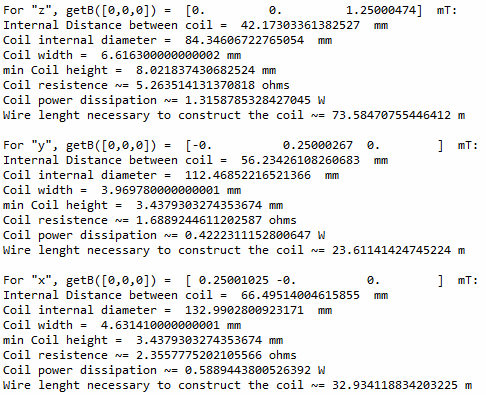
\includegraphics[width=0.67\textwidth]{./img/simulacao/console.png}
     \caption*{Fonte: Autor.}\label{fig:cons}
\end{figure}

As informações mostradas representam respectivamente para cada bobina:

\begin{itemize}
    \item O campo estimado no centro da estrutura em $mT$.
    \item A distância entre os dois enrolamentos de cada bobina de Helmholtz em mm.
    \item O diâmetro interno dos enrolamentos de cada bobina de Helmholtz em mm.
    \item A espessura do enrolamento (Citado na figura \ref{fig:model}) da bobina de Helmholtz em mm.
    \item A altura do enrolamento (Citado na figura \ref{fig:model}) da bobina de Helmholtz em mm.
    \item A resistência estimada para cada bobina de Helmholtz em $\Omega$.
    \item A potência dissipada por cada bobina de Helmholtz em W.
    \item A quantidade de fio em metros necessária para construir cada bobina.
\end{itemize}

Na tabela \ref{tab:paramSim} são listados os parâmetros calculados para o desenvolvimento do suporte dos enrolamentos das bobinas de Helmholtz, raio dos enrolamentos de cada bobina, espessura do enrolamento e altura do enrolamento de cada bobina de Helmholtz.

\begin{table}[H]
    \centering
    \caption{Parâmetros retirados do simulador}
    \begin{tabular}{ |p{2.5cm}|p{2cm}|p{3.9cm}|p{4.4cm}|}
     \hline
     \textbf{Bobina} & \textbf{Raio} & \textbf{Espessura vertical}& \textbf{Espessura horizontal} \\
     \hline
     Interna & 42.5 mm & 6.6 mm & 9.65 mm \\
     Intermediária & 56.15 mm & 4 mm & 5.5 mm \\
     Externa & 66.5 mm & 4.65 mm & 5.5 mm \\
     \hline
    \end{tabular}
    \label{tab:paramSim}
\end{table}


\subsection{Modelos 3D}

Para evitar problemas de desalinhamento e de montagem mecânica optou-se pela confecção de uma peça única, onde as três bobinas seriam enroladas.

O modelo para o suporte das bobinas é mostrado na figura \ref{fig:mod3D}, desenhado no software solidWorks \cite{solidWorks}. Nesse modelo é possível observar cinco orifícios na visão superior. Quatro desses orifícios serão utilizados para a fixação do suporte do sensor do sistema e o transdutor a ser avaliado, sendo o orifício central utilizado para a passagem de fios de conexão com os sensores.


\begin{figure}[H]
    \centering
     \caption{Modelo do suporte das bobinas.}
     \subfloat[Visão lateral.]{%
       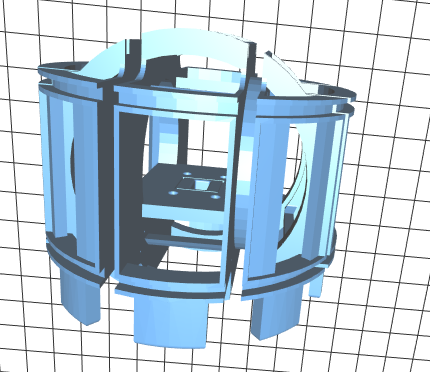
\includegraphics[width=0.3\textwidth]{./img/modelos3D/3DHC model.png}
     }
     \subfloat[Visão inferior.]{%
       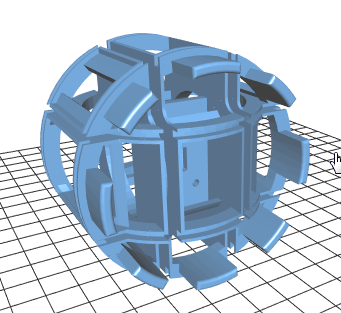
\includegraphics[width=0.3\textwidth]{./img/modelos3D/3DHC model 2.png}
     }
     \subfloat[Visão superior.]{%
       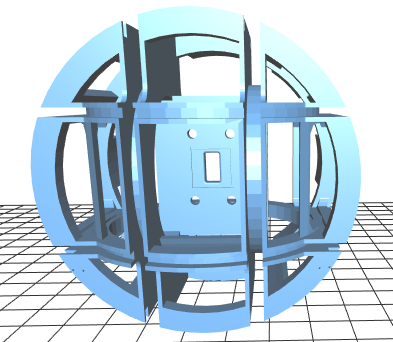
\includegraphics[width=0.3\textwidth]{./img/modelos3D/3DHC model 3.png}
     }
    % \hfill
     \caption*{Fonte: Autor.}\label{fig:mod3D}
\end{figure}

A seguir o modelo do suporte do sensor do sistema e do transdutor produzido pela SAL. O modelo pode ser visto na figura \ref{fig:sups}, sendo os quatro pilares centrais o suporte do sensor do sistema e a estrutura planar mais externa o suporte do transdutor a ser avaliado.

\begin{figure}[H]
    \centering
     \caption{Modelo do suporte do sensor.}
     \subfloat[Visão superior]{%
        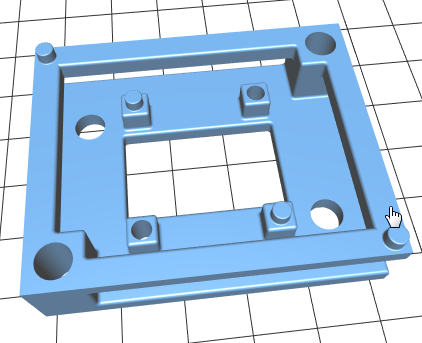
\includegraphics[width=0.5\textwidth]{./img/modelos3D/sensor support.png}
     }
     \subfloat[Visão inferior]{%
        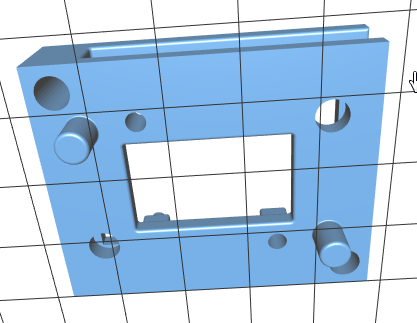
\includegraphics[width=0.5\textwidth]{./img/modelos3D/sensor support 2.png}
     }
    % \hfill
     \caption*{Fonte: Autor.}\label{fig:sups}
\end{figure}

Para a fixação do suporte do sensor foram confeccionados rebites de diversos tamanhos, que possibilitavam diferentes pressões para fixar o suporte do sensor e transdutor no suporte das bobinas. O modelo dos rebites pode ser observado na figura \ref{fig:reb}.

\begin{figure}[H]
    \centering
     \caption{Modelo dos rebites.}
     \subfloat[Visão inferior]{%
        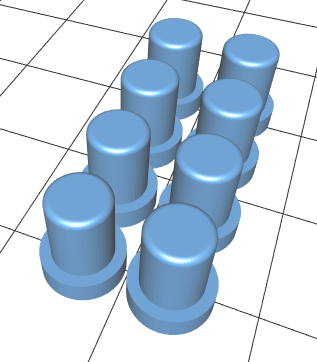
\includegraphics[width=0.32\textwidth]{./img/modelos3D/pegs example 1.png}
     }
     \subfloat[Visão superior]{%
        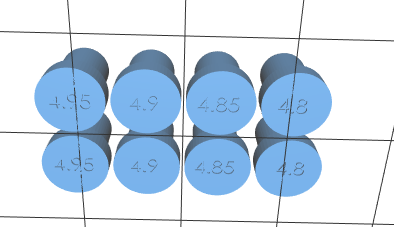
\includegraphics[width=0.68\textwidth]{./img/modelos3D/pegs example 2.png}
     }
    % \hfill
     \caption*{Fonte: Autor.}\label{fig:reb}
\end{figure}

Para uma menor interação das bobinas com possíveis estruturas metálicas onde a bobina seria apoiada foi desenvolvido o modelo de um tripé que possa suportar as bobinas a uma altura equivalente a 20 cm, valor definido pelo orientador do projeto na empresa. O modelo deste tripé pode ser observado na figura \ref{fig:trip}.

\begin{figure}[H]
    \centering
     \caption{Modelo do tripé.}
     \subfloat[]{%
        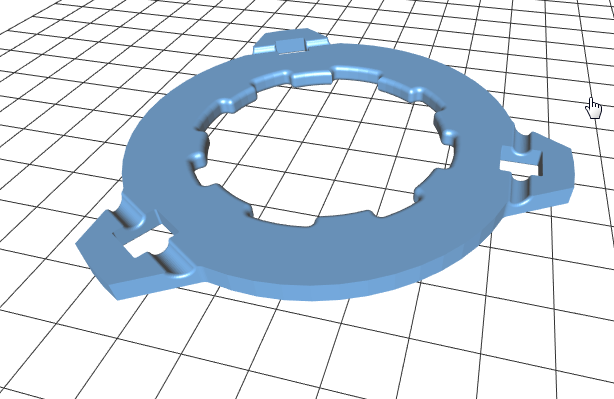
\includegraphics[width=0.4\textwidth]{./img/modelos3D/coils support 1.png}
     }
     \subfloat[]{%
        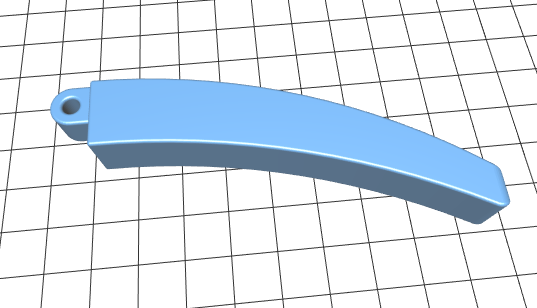
\includegraphics[width=0.4\textwidth]{./img/modelos3D/coil support 2.png}
     }
     \subfloat[]{%
        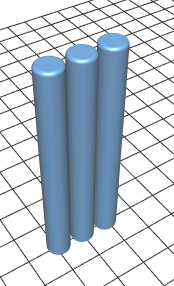
\includegraphics[width=0.15\textwidth]{./img/modelos3D/coil support 3.png}
     }
    % \hfill
     \caption*{Fonte: Autor.}\label{fig:trip}
\end{figure}

\section{Processamento de dados}

\subsection{Matriz de rotação}

É inerente da medição o desalinhamento entre a direção do campo gerado pelas bobinas e a direção de indução magnética medida pelo sensor, pois o mesmo estará de alguma forma com seu eixos de medição deslocados dos eixos do campo gerado. Para resolver esse desalinhamento foi desenvolvida uma matriz de rotação que alinha o campo medido pelo sensor. A seguir é descrita a matriz de rotação, o cálculo em \textit{python} pode ser visto no apêndice A.

As informações conhecidas a respeito da geração dos campos magnéticos e da medição é:
\begin{itemize}
    \item Corrente elétrica injetada nas bobinas de Helmholtz, $I$.
    \item Valor de campo de indução magnética gerado apenas pelas bobinas de Helmholtz medido com o sensor no centro da estrutura, este chamado de $M$. 
    \item Razão entre corrente injetada e campo de indução magnética produzida por cada bobina, chamada de $Cb$.
\end{itemize}

Na equação \ref{eq:rot} é apresentada a relação entre as medidas obtidas e as medidas geradas após a transformação de rotação. Assumindo que $M$ está desalinhado em relação ao campo gerado por $I$ e representa a medida desse mesmo campo. A relação entre as matrizes $I$ e $M$, sem modificação da norma será chamada de $\mu$. A matriz $Cb$ é uma matriz que transforma as correntes $I$ em um valor correspondente de indução magnética, isso é feito através do produto interno entre $Cb$ e $I$.

\begin{gather}
\label{eq:rot}
 \begin{bmatrix} I\cdot C_b \end{bmatrix}_{3x1}
 =
  \begin{bmatrix}
   \mu
   \end{bmatrix}_{3x3}
 \begin{bmatrix} M \end{bmatrix}_{3x1}
\end{gather}

Sendo:

\begin{gather}
\label{eq:mI}
 \begin{bmatrix} I \end{bmatrix}_{3x1}
 =
  \begin{bmatrix}
   I_x \\
   I_y \\
   I_z
   \end{bmatrix}
\end{gather}


\begin{gather}
\label{eq:mM}
 \begin{bmatrix} M \end{bmatrix}_{3x1}
 =
  \begin{bmatrix}
   M_{xb} - M_{xa} \\
   M_{yb} - M_{ya} \\
   M_{zb} - M_{za}
   \end{bmatrix}
 =
  \begin{bmatrix}
   M_x \\
   M_y \\
   M_z
   \end{bmatrix}
\end{gather}

\begin{gather}
\label{eq:mC}
 \begin{bmatrix} C_b \end{bmatrix}_{3x1}
 =
  \begin{bmatrix}
   C_{bx} \\
   C_{by} \\
   C_{bz}
   \end{bmatrix}
\end{gather}

\begin{gather}
\label{eq:mu}
 \begin{bmatrix} \mu \end{bmatrix}_{3x3}
 =
  \begin{bmatrix}
   \mu_{x1} & \mu_{y1} & \mu_{z1} \\
   \mu_{x2} & \mu_{y2} & \mu_{z2} \\
   \mu_{x3} & \mu_{y3} & \mu_{z3} \\
   \end{bmatrix}
\end{gather}

Como o objetivo é lidar apenas com o campo gerado pelas bobinas, é feito primeiramente a medição do campo do ambiente, sem nenhuma bobina ligada, este chamado de $M_a$, outra medida $M_b$ com as bobinas ligadas. A subtração dessas duas medidas leva a medição do campo gerado apenas pelas bobinas.

Há nove incógnitas e apenas um direção linearmente independente. Todavia isto pode ser resolvido obtendo-se três medidas em três direções independentes. Obtendo-se três vezes mais informação é possível a resolução do sistema. Nas equações \ref{eq:rotA} e \ref{eq:rotB} é possível observar o sistema formado por essas três medições.

\begin{gather}
\label{eq:rotA}
 \begin{bmatrix} I_1\cdot C_{b}  & I_2\cdot C_{b}  & I_3\cdot C_{b}  \end{bmatrix}_{3x3}
 =
  \begin{bmatrix}
   \mu
   \end{bmatrix}_{3x3}
 \begin{bmatrix} M_1& M_2 & M_3 \end{bmatrix}_{3x3}
\end{gather}


\begin{gather}
\label{eq:rotB}
 \begin{bmatrix} I_{1x}\cdot C_{bx} & I_{2x}\cdot C_{bx} & I_{3x}\cdot C_{bx} \\
 I_{1y}\cdot C_{by} & I_{2y}\cdot C_{by} & I_{3y}\cdot C_{by} \\
 I_{1z}\cdot C_{bz} & I_{2z}\cdot C_{bz} & I_{3z}\cdot C_{bz} \\
 \end{bmatrix}
 =
   \begin{bmatrix}
   \mu_{x1} & \mu_{y1} & \mu_{z1} \\
   \mu_{x2} & \mu_{y2} & \mu_{z3} \\
   \mu_{x3} & \mu_{y2} & \mu_{z3} \\
   \end{bmatrix}
    \begin{bmatrix}
   M_{1x} & M_{2x} & M_{3x} \\
   M_{1y} & M_{2y} & M_{3y} \\
   M_{1z} & M_{2z} & M_{3z} \\
   \end{bmatrix}
\end{gather}

$Cb$ é a razão entre o campo gerado pela bobina e a corrente na mesma. Essa matriz pode ser encontrado através de um procedimento simples:

\begin{itemize}
    \item Mede-se o campo no centro da bobina, sabendo que este é o campo atual naquele ponto, chamando a medida de $M_{cb1}$
    \item Aplica-se uma corrente $I_{cb}$ conhecida na bobina e mede-se o campo no centro da bobina outra vez, sem movimentar o sensor de lugar, chamando esta medida de $M_{cb2}$
\end{itemize}

A intensidade do campo gerado $Cg$ pela bobina será exatamente a norma da diferença entre $M_{cb2}$ e $M_{cb1}$. Sabendo a corrente $I_{cb}$ é possível determinar-se $Cb$ fazendo a razão entre $Cg$ e $I_{cb}$, o que pode ser observado na equação \ref{eq:cbfrac}.

\begin{equation}
    \label{eq:cbfrac}
    C_b = \frac{C_g}{I_{cb}}
\end{equation}

Sendo conhecidas as matrizes $I$, $M$ e $Cb$ é possível determinar $\mu$ através da resolução do sistema linear. O código de cálculo da chamada matriz de rotação $\mu$ pode ser observado no apêndice A.

\subsection{Aumento da relação Sinal Ruído através de média}

O ruído RMS do sensor utilizado é de 0.15 $\mu$T \cite{mcc3416}. Essa característica pode ser melhorada através de média, dado que os campos gerados devem permanecer estáticos do começo ao fim da medida. A equação \ref{eq:SRNn1} \cite{noiseRedArt} descreve o aumento da relação sinal ruído de uma média de medidas com número N ($SRN_N$) em relação a apenas uma medida ($SRN_1$).

\begin{equation}
    \label{eq:SRNn1}
    SRN_N = \sqrt{N}\cdot SRN_1
\end{equation}

Foi feito um teste empírico para observar qual seria o melhor valor de medidas N sem que ocorresse degradação do funcionamento do equipamento.

Sendo 1 $\mu$T o valor da resolução de sinal, na equação \ref{eq:SRN1}, é possível observar a relação sinal ruído para apenas uma amostra do sensor MMC3416. Esse valor é utilizado para o cálculo da relação sinal ruído com 30 amostras na equação \ref{eq:SRNN}. Há um ganho na SRN da medida de 6,66 para 36,5.


\begin{equation}
    \label{eq:SRN1}
    SRN_1 = \frac{1}{0.15} = 6.666
\end{equation}

\begin{equation}
    \label{eq:SRNN}
    SRN_N = \sqrt{30}\cdot 6.666 = 36.5
\end{equation}

Utilizando a nova relação sinal ruído encontrada, é possível calcular-se o novo ruído RMS de cada medida, o que pode ser observado na equação \ref{eq:RMSn}. O valor encontrado de 0,027 μT é 5,55 vezes menor que o valor anteriormente citado. Assim, se obtém um ganho de exatidão das medidas sem a degradação do desempenho do equipamento.

\begin{equation}
    \label{eq:RMSn}
    RMS_{noise} = \frac{1}{36.5} = 0.027 \mu T
\end{equation}
\chapter{Resultados}

\section{Placas de Circuito Impresso}

As placas de circuito impresso foram produzidas em uma empresa externa \cite{euroC}, utilizando os arquivos gerados no programa EAGLE 7.1 \cite{EagleWiki}. 

A placa para o encaixe do sensor pode ser obsevada na figura \ref{fig:pcbSensor}. A importância dessa placa é a de alinhamento do sensor com a região de interesse no centro da estrutura em conjunto com o suporte do sensor. Emprega um conector que possui boa fixação para diminuir eventuais problemas de conexão. 

A estratégia utilizada no cabo produzido dessa placa foi a de transmitir paralelamente a cada fio de sinal, um fio de referência, trançando levemente os dois cabos para uma diminuição de ruído irradiado. Assim, esse par de fios reduz o efeito produzido pelas correntes de modo comum, onde o campo gerado pelo cabo do sinal é cancelado pelo campo gerado pelo cabo de referência que o acompanha.

\begin{figure}[H]
    \centering
     \caption{Resultado da PCI do sensor.}
     \subfloat[Visão superior.]{%
       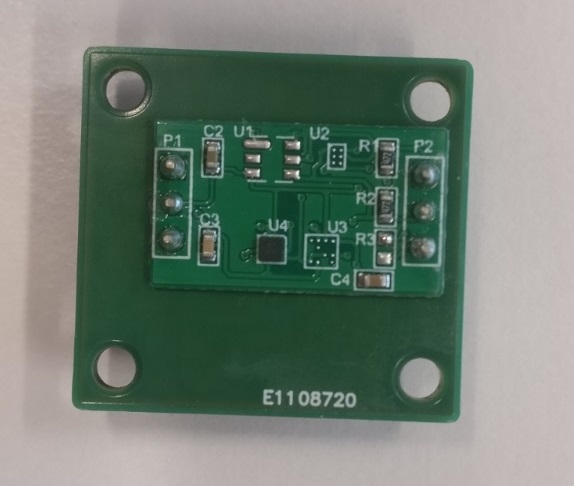
\includegraphics[width=0.51\textwidth]{./img/PCBs/placaSensor.jpg}
     }
     \subfloat[Visão inferior.]{%
       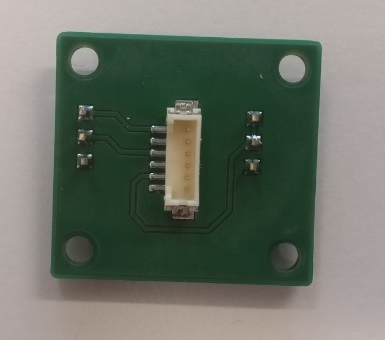
\includegraphics[width=0.49\textwidth]{./img/PCBs/placaSensor1.jpg}
     }
    % \hfill
     \caption*{Fonte: Autor.}\label{fig:pcbSensor}
\end{figure}

A PCI principal do sistema, na qual estão conectados o computador, a fonte, o sensor e as bobinas, é mostrada na figura \ref{fig:pbcMain}. Nessa, a preocupação maior era com a solda dos componentes SMD, pois esse procedimento seria feito de forma manual. Nesse caso, um \textit{stencil} foi utilizado juntamente com um forno elétrico doméstico, facilitando o processo de inserção e soldagem da placa.

Os componentes estão distribuídos espaçadamente na placa para melhor manuseio. A distribuição foi pensada para facilitar as conexões necessárias e uma possível manutenção. Na figura \ref{fig:hardwareSistema} é possível observar o sistema montado com sensor e microcontrolador conectados na placa principal.

\begin{figure}[H]
    \centering
     \caption{Resultado da PCI do sistema}
     \subfloat[Visão superior]{%
       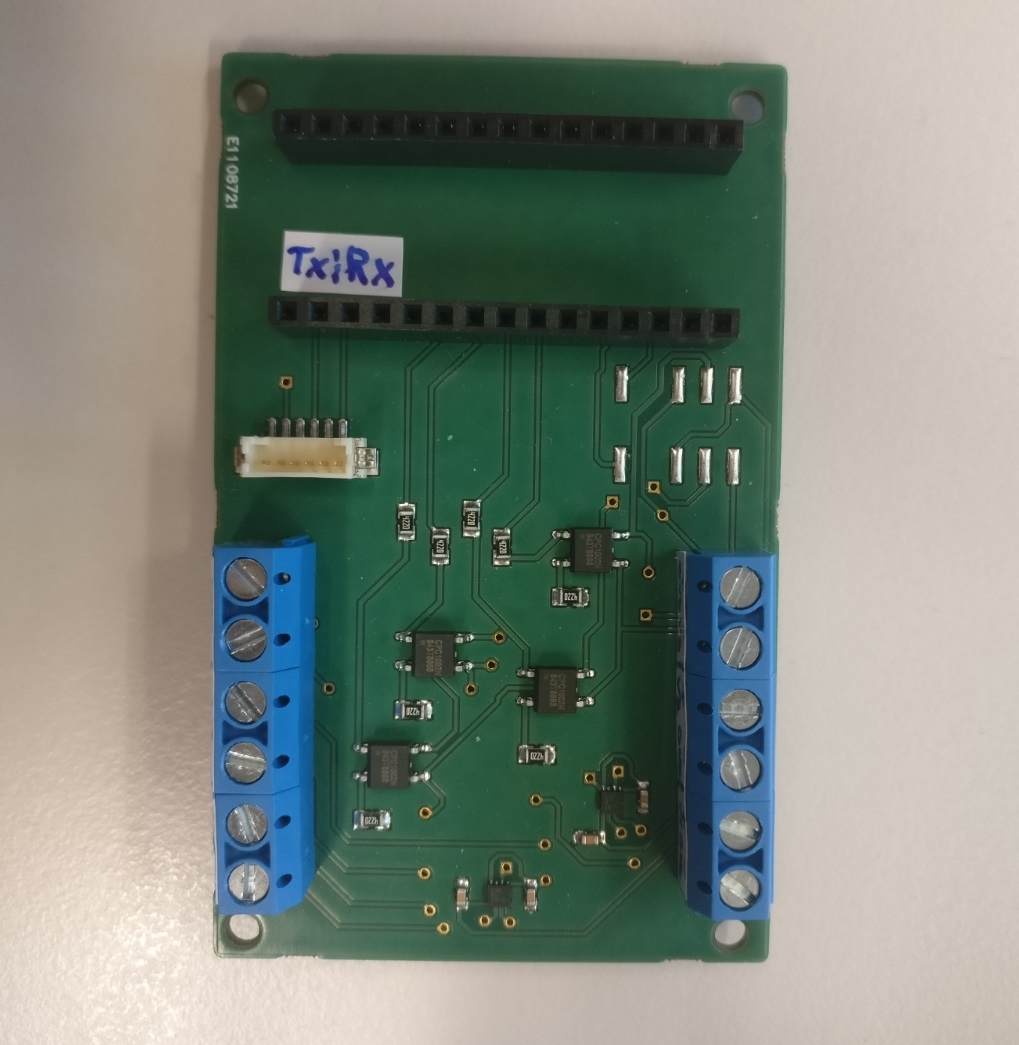
\includegraphics[width=0.51\textwidth]{./img/PCBs/placaMain1.jpg}
     }
     \subfloat[Visão inferior]{%
       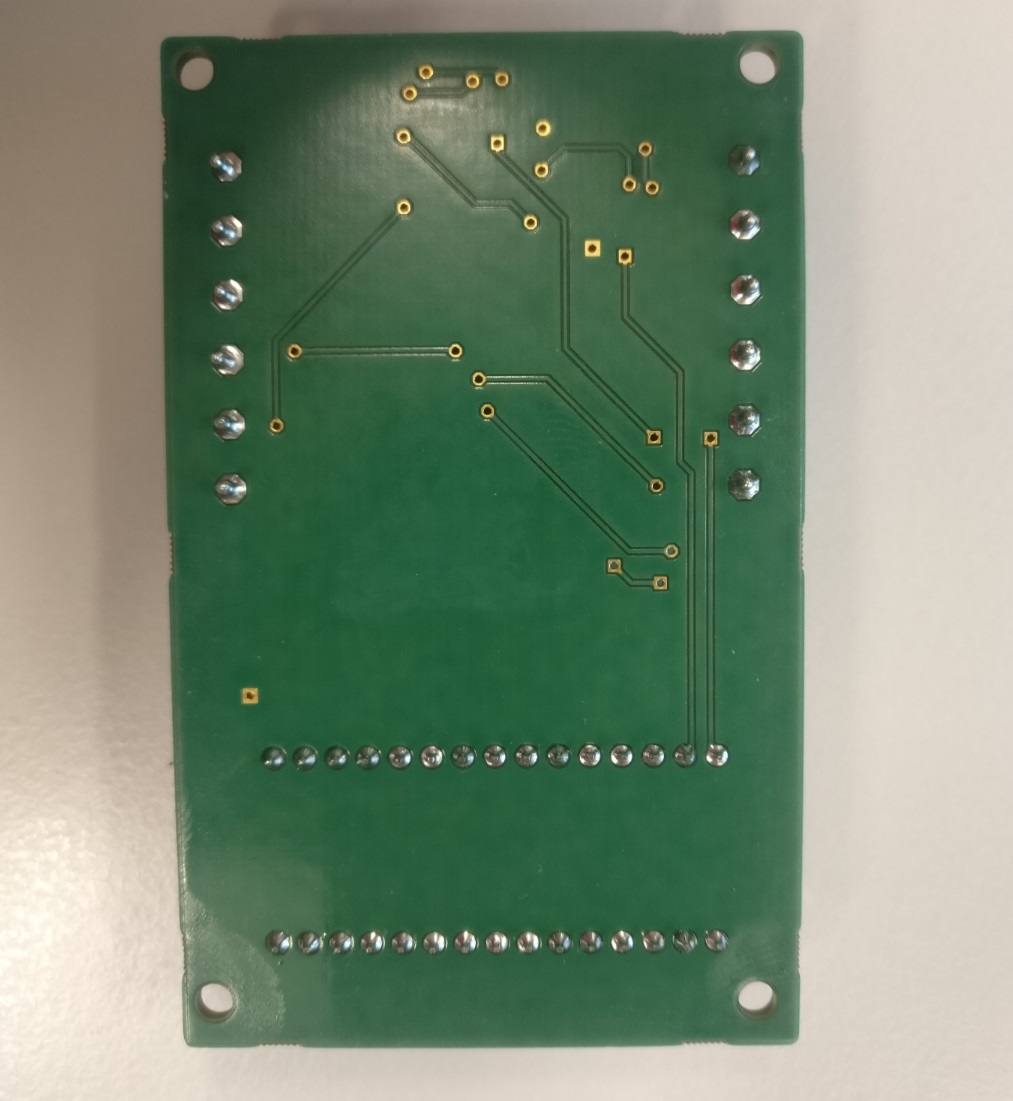
\includegraphics[width=0.48\textwidth]{./img/PCBs/placaMain.jpg}
     }
    % \hfill
     \caption*{Fonte: Autor.}\label{fig:pbcMain}
\end{figure}

\begin{figure}[H]
    \centering
     \caption{Hardware montado.}
     \includegraphics[width=0.55\textwidth]{./img/PCBs/placaMontada.jpg}
     \caption*{Fonte: Autor.}\label{fig:hardwareSistema}
\end{figure}

\section{Impressões 3D}

Para que os resultados obtidos nas simulações fossem alcançados, a impressão das peças tridimensionais deveria ter a maior precisão possível. As impressões realizadas para todas as peças exceto o tripé contam com uma precisão de 0,05 $\mu m$ o que faz desprezível qualquer problema mecânico relacionado a precisão da impressão.

Os resultados das impressões do suporte do sensor e transdutor pode ser observado na figura \label{fig:supsenim} e dos rebites na figura \label{fig:rebim}. Os rebites tem diferença de 50 μm entre seus diâmetros, possibilitando diferentes pressões de fixação do suporte do sensor e transdutor.

\begin{figure}[H]
    \centering
     \caption{Suporte do sensor.}
     \includegraphics[width=0.55\textwidth]{./img/impressoes3D/suporte_sensor.jpg}
     \caption*{Fonte: Autor.}\label{fig:supsenim}
\end{figure}

\begin{figure}[H]
    \centering
     \caption{Resultado da impressão dos rebites.}
     \includegraphics[width=0.55\textwidth]{./img/impressoes3D/rebites.jpg}
     \caption*{Fonte: Autor.}\label{fig:rebim}
\end{figure}

Na impressão do tripé para o suporte das bobinas a precisão da impressora não era relevante para o resultado. O resultado da impressão do tripé pode ser observado na figura \ref{fig:tripim}, o centro do tripé foi projetado para que se encaixe perfeitamente ao suporte das bobinas, com o desenho formado pelos "pés" do suporte. A estrutura impressa do suporte das bobinas pode ser observada na figura \ref{fig:bob}.

\begin{figure}[H]
    \centering
     \caption{Impressão do tripé.}
     \includegraphics[width=0.5\textwidth]{./img/impressoes3D/tripe.jpg}
     \caption*{Fonte: Autor.}\label{fig:tripim}
\end{figure}

\begin{figure}[H]
    \centering
     \caption{Impressão do suporte para as bobinas 3D}
     \includegraphics[width=0.5\textwidth]{./img/impressoes3D/bobiba1.jpg}
     \caption*{Fonte: Autor.}\label{fig:bob}
\end{figure}

Na figura \ref{fig:sensup} é possível observar a peça de suporte do sensor encaixada ao suporte das bobinas. A fixação é feita através dos rebites, os quais dão pressão mecânica, o sensor fica posicionado no centro da estrutura, não havendo problemas de movimentação durante as medições.

\begin{figure}[H]
    \centering
     \caption{Encaixe do suporte do sensor}
     \subfloat[]{%
        
     \includegraphics[width=0.45\textwidth]{./img/impressoes3D/encaixe_suporte_sensor.jpg}
     }
     \subfloat[]{%
     \includegraphics[width=0.38\textwidth]{./img/impressoes3D/encaixe_suporte_sensor 2.png}
     }
     \caption*{Fonte: Autor.}\label{fig:sensup}
\end{figure}


\section{Enrolamento das bobinas}

O enrolamento das bobinas foi realizado de forma simples, utilizando uma morsa de bancada, uma chave de fenda e o próprio rolo de fio. Foi possível gerar uma tensão sobre o fio ao ser esticado, mostrado na figura \ref{fig:morsa} (a). Esse fio ao ser enrolado no suporte das bobinas com essa tensão se encaixa perfeitamente no suporte das bobinas, permitindo que a geometria dos enrolamentos fique quase igual à geometria utilizada no simulador, o que é importante para que a indução real gerada pelas bobinas seja a mais próxima possível da indução verificada nas simulações. Na figura \ref{fig:morsa} (b) é possível observar as bobinas enroladas no suporte.

\begin{figure}[H]
    \centering
     \caption{Enrolamento das bobinas}
     \subfloat[]{%
        
     \includegraphics[width=0.45\textwidth]{./img/resultados/morsa.jpg}
     }
     \subfloat[]{%
     \includegraphics[width=0.415\textwidth]{./img/resultados/bobinas2.jpg}
     }
     \caption*{Fonte: Autor.}\label{fig:morsa}
\end{figure}


\section{Caracterização das bobinas}

Na figura \ref{fig:final} pode ser visualizado o equipamento montado e integrado. Os cabos vindos da fonte de potência são conectados em um lado da placa do sistema, a corrente por eles transmitida passa pelas pontes H, uma para cada canal, saindo pelo outro lado da placa que está conectado diretamente às bobinas. Há uma conexão entre o sensor localizado no meio da estrutura de suporte das bobinas e a placa principal do sistema, feita por um cabo de pares levemente trançados. O microcontrolador da placa do sistema é conectado ao computador através de um cabo USB. A aquisição de dados é recebida por um computador, o qual processa as medidas para que sejam ajustadas para a posição correta.


\begin{figure}[H]
    \centering
     \caption{Equipamento montado e integrado}
     \includegraphics[width=1\textwidth]{./img/resultados/resultSystem.jpg}
     \caption*{Fonte: Autor.}\label{fig:final}
\end{figure}

Na análise das bobinas foi utilizado o sensor magnético MMC3416 posicionado no centro da estrutura de suporte. Então, as medidas em $\muT$ dos eixos x, y e z são enviadas para um computador. As medidas enviadas estão em $\muT$, com medidas em x, y e z respectivamente em cada linha recebida.

\subsection{Bobina interna}

A bobina mais interna, também chamada de bobina principal z, é a bobina que gera o campo mais intenso, com maior número de enrolamentos e maior quantidade de fio. Em comparação com os outros enrolamentos, este tem a maior resistência e indutância. Nas figuras \ref{fig:ResIndIn} e \ref{fig:CurFieldIn} podem ser vistos, para essa bobina, os valores medidos de tensão, corrente, indução magnética, resistência e indutância.

\begin{figure}[H]
    \centering
     \caption{Medidas de resistência e indutância na bobina interna}
     \subfloat[Valor da resistência medida ($\Omega$)]{%
        \includegraphics[width=0.25\textwidth]{./img/bob/innerCoilResistance.jpg}
     }
     \subfloat[Valor da indutância medida (mH)]{%
        \includegraphics[width=0.24\textwidth]{./img/bob/innerCoilInductance.jpg}
     }
    % \hfill
     \caption*{Fonte: Autor.}\label{fig:ResIndIn}
\end{figure}


\begin{figure}[H]
    \centering
     \caption{Estimação do campo gerado pela bobina interna}
     \subfloat[Tensão e corrente da fonte]{%
        \includegraphics[width=0.35\textwidth]{./img/bob/innerCoilCurrent.jpg}
     }
     \subfloat[Valores de campo recebidos no computador]{%
        \includegraphics[width=0.23\textwidth]{./img/bob/innerCoilField.jpg}
     }
    % \hfill
     \caption*{Fonte: Autor.}\label{fig:CurFieldIn}
\end{figure}


\subsection{Bobina intermediária e externa}

As medidas de resistência e campo gerado pelas bobinas intermediária e externa podem ser vistas nas figura \ref{fig:ResIndMd}, \ref{fig:CurFieldMd}, \ref{fig:ResIndEx} e \ref{fig:CurFieldEx}.

\begin{figure}[H]
    \centering
     \caption{Medidas de resistência e indutância na bobina intermediária}
     \subfloat[Valor da resistência medida ($\Omega$)]{%
        \includegraphics[width=0.26\textwidth]{./img/bob/midCoilResistance.jpg}
     }
     \subfloat[Valor da indutância medida (mH)]{%
        \includegraphics[width=0.24\textwidth]{./img/bob/midCoilInductance.jpg}
     }
    % \hfill
     \caption*{Fonte: Autor.}\label{fig:ResIndMd}
\end{figure}

\begin{figure}[H]
    \centering
     \caption{Estimação do campo gerado pela bobina intermediária}
     \subfloat[Tensão e corrente da fonte]{%
        \includegraphics[width=0.35\textwidth]{./img/bob/midCoilCurrent.jpg}
     }
     \subfloat[Valores de campo recebidos no computador]{%
        \includegraphics[width=0.245\textwidth]{./img/bob/midCoilField.jpg}
     }
    % \hfill
     \caption*{Fonte: Autor.}\label{fig:CurFieldMd}
\end{figure}


\begin{figure}[H]
    \centering
     \caption{Medidas de resistência e indutância na bobina externa}
     \subfloat[Valor da resistência medida ($\Omega$)]{%
        \includegraphics[width=0.25\textwidth]{./img/bob/externalCoilResistance.jpg}
     }
     \subfloat[Valor da indutância medida (mH)]{%
        \includegraphics[width=0.235\textwidth]{./img/bob/externalCoilInductance.jpg}
     }
    % \hfill
     \caption*{Fonte: Autor.}\label{fig:ResIndEx}
\end{figure}

\begin{figure}[H]
    \centering
     \caption{Estimação do campo gerado pela bobina interna}
     \subfloat[Tensão e corrente da fonte]{%
        \includegraphics[width=0.35\textwidth]{./img/bob/externalCoilCurrent.jpg}
     }
     \subfloat[Valores de campo recebidos no computador]{%
        \includegraphics[width=0.23\textwidth]{./img/bob/externalCoilField.jpg}
     }
    % \hfill
     \caption*{Fonte: Autor.}\label{fig:CurFieldEx}
\end{figure}
Fazendo uma breve comparação entre os valores teóricos e estimados com os valores medidos, chegaram-se aos erros encontrados na figura \ref{fig:err}, essas informações são melhores apresentadas nas tabelas \ref{tab:intCoil}, \ref{tab:midCoil} e \ref{tab:extCoil}.
Com base nessas informações é possível considerar que os métodos utilizados permitiram gerar um campo em cada bobina na direção desejada, alinhados com o sensor. Há um erro de amplitude menor que 2\% em todas as bobinas, o que é aceitável para este projeto. Os valores de resistência ficaram bem diferentes do estimado. Porém, a influência desse parâmetro não afeta de forma significativa o equipamento e pode ser desprezada.

A indutância foi medida para possíveis alterações no funcionamento das bobinas, não sendo relevante para este trabalho. 

\begin{figure}[H]
    \centering
     \caption{Erros encontrados no módulo de campo da bobina }
     \includegraphics[width=0.8\textwidth]{./img/bob/fieldErr.png}
     \caption*{Fonte: Autor.}\label{fig:err}
\end{figure}

\begin{table}[H]
    \centering
    \caption{Informações da bobina (Interna)}
    \begin{tabular}{|c|c|c|c|}
     \hline
     \textbf{Parâmetro} & \textbf{Valores estimados} & \textbf{Valores medidos} & \textbf{erro}\\
     \hline
     Resistência&  5.26 $\Omega$  & 5.69 $\Omega$ & 8.09 \% \\ 
     Campo induzido &   1250.00 $\mu$T  & 1236.47 $\mu$T & -1.08 \% \\ \hline
     
    \end{tabular}
    \label{tab:intCoil}
\end{table}

\begin{table}[H]
    \centering
    \caption{Informações da bobina (Intermediária)}
    \begin{tabular}{|c|c|c|c|}
     \hline
     \textbf{Parâmetro} & \textbf{Valores estimados} & \textbf{Valores medidos} & \textbf{erro}\\
     \hline
     Resistência&  1.69 $\Omega$  & 1.93 $\Omega$ & 14.27 \% \\ 
     Campo induzido &  250.00 $\mu$T  & 250.36 $\mu$T & 0.15 \% \\ \hline
     
    \end{tabular}
    \label{tab:midCoil}
\end{table}

\begin{table}[H]
    \centering
    \caption{Informações da bobina (Exterior)}
    \begin{tabular}{|c|c|c|c|}
     \hline
     \textbf{Parâmetro} & \textbf{Valores estimados} & \textbf{Valores medidos} & \textbf{erro}\\
     \hline
     Resistência&  2.36 $\Omega$  & 2.59 $\Omega$ & 9.93 \% \\ 
     Campo induzido &   250.00 $\mu$T  & 254.12 $\mu$T & 1.65 \% \\ \hline
     
    \end{tabular}
    \label{tab:extCoil}
\end{table}

Dois testes foram feitos para determinar o comportamento do campo gerado através da observação de uma bussola. No primeiro teste foi feito um \textit{script} em \textit{python} que compensava o campo magnético terrestre e em seguida gerava um campo circular no plano xy. O efeito desse sinal magnético sendo aplicado na bussola fazia com que a mesma ficasse com seu ponteiro girando de forma circular e com velocidade angular constante, na faixa de alguns Hertz.

Observando-se esse primeiro teste era possível determinar se o sistema estava controlando as bobinas da maneira correta, não vendo nenhum tipo de mudança abrupta na movimentação da bússola por exemplo.

Outro teste realizado foi a compensação total do campo magnético da terra. A bussola era sensível o suficiente para detectar campos de cerca de 2 $\mu T$. Foi feito um \textit{script} em \textit{python} que apenas compensava o campo magnético terrestre. Após compensado a bussola era colocada no centro da região de campo uniforme. Com a bússola no centro da estrutura um imã era aproximado fazendo com que a mesma apontasse para o imã. Como não havia nenhum campo resultante, assim que o imã era afastado da bussola, a mesma permanecia apontada para a direção que o imã estava. Após esse teste a corrente das bobinas eram desligadas e a bússola voltava a apontar para o norte terrestre, mostrando que o sistema era capaz de anula o campo magnético terrestre. Na figura \ref{fig:compass} pode-se observar uma ilustração da bússola no centro da estrutura.


\begin{figure}[H]
    \centering
     \caption{Ilustração da bússola no centro da estrutura das bobinas}
     \includegraphics[width=0.4\textwidth]{./img/compass.png}
     \caption*{Fonte: Autor.}\label{fig:compass}
\end{figure}
\chapter{Conclusão}

Foi desenvolvido um equipamento capaz de gerar um campo homogêneo e uniforme em uma determinada região para análise de sensores magnéticos. O campo é gerado com o emprego de três bobinas de Helmholtz, dispostas nos eixos x, y e z.

O projeto das bobinas foi realizado com uma biblioteca de cálculo de campo em python \cite{magpy2020}, a qual utiliza soluções analíticas para o cálculo do campo gerado pelas bobinas de Helmholtz, possibilitando um projeto para qualquer requisito de bobina. Uma vez projetadas as bobinas, uma estrutura mecânica foi desenvolvida e impressa atendendo os requisitos de precisão necessários.

O sistema eletrônico desenvolvido utiliza um padrão simples de comunicação com um computador, tornando o controle das bobinas e aquisição de dados independente de um software específico ou sistema operacional.

A integração do sistema é feita por módulos independentes, tanto eletrônicos como mecânicos, o que permite a reutilização de partes do sistema e facilita a manutenção.

Todos os requisitos de projeto, colocados nos objetivos deste trabalho, foram alcançados, estando o sistema em uso na Silicon Austria Labs, onde foi desenvolvido.

Como sugestão de trabalho futuro poderia ser desenvolvido o controle de campos dinâmicos, o que levaria em conta a indutância e os tempos de escrita e leitura desses campos, possibilitando a geração de sinais magnéticos no centro do equipamento, aumentando suas aplicações.  Outra sugestão é o desenvolvimento de uma interface gráfica mais intuitiva e amigável para uso no computador, facilitando o uso do equipamento.

% ----------------------------------------------------------
% ELEMENTOS PÓS-TEXTUAIS 
% ----------------------------------------------------------
\postextual

% ----------------------------------------------------------
% REFERÊNCIAS BIBLIOGRÁFICAS
% ----------------------------------------------------------
\bibliography{./bib/bibTCC}

% ----------------------------------------------------------
% GLOSSARIO
% ----------------------------------------------------------
% Consulte o manual da classe abntex2 para orientações sobre o glossário.
%\glossary

% ----------------------------------------------------------
% APÊNDICES
% ----------------------------------------------------------
%\begin{apendicesenv}
\apendices
\chapter{Código do cálculo da matrix de rotação}

\begin{minted}[
frame=lines,
framesep=1mm,
baselinestretch=0.5,
fontsize=\footnotesize,
linenos
]{python}

def rotationMatrixCalculator(visaObj, serialObj, teorethicalValue):
    
    # Rotation matrix, to align the measurements with the Coils axis
    fData = getMeasurement(serialObj)    
    # print(fData)
    
    # buffer to do the rotation matrix measurements
    bufferData = np.zeros((4,3))
    
    # Assuming that the measurement is precise enough
    bufferData[0,0] = fData[0]
    bufferData[0,1] = fData[1]
    bufferData[0,2] = fData[2]
    
    # Setting the voltage for the power supply
    setPowerSupplyAllChVoltage(visaObj, 4)
    
    # Current used in the coils to make the relationship between current and field measured
    baseCurrent = 400 #mA
    
    # Code to get the measurement information for the rotation matrix
    for i in range(3,0,-1):
        
        setPowerSupplyChCurrent(visaObj, i, baseCurrent/1000)
        sleep(0.1)
        
        fData = getMeasurement(serialObj)
        
        setPowerSupplyChCurrent(visaObj, i, 0)
        sleep(0.1)    
        
        bufferData[i,0] = fData[0] - bufferData[0,0]
        bufferData[i,1] = fData[1] - bufferData[0,1]
        bufferData[i,2] = fData[2] - bufferData[0,2]
        
    # Doing a linear relationship between the Current set in the coil and the Field measured with this 
    ch1Field = np.linalg.norm(bufferData[1,:])
    ch1Current = baseCurrent
    
    ch2Field = np.linalg.norm(bufferData[2,:])
    ch2Current = baseCurrent
    
    ch3Field = np.linalg.norm(bufferData[3,:])
    ch3Current = baseCurrent
    
    
    CurrentToField = np.zeros((3,1))
    FieldToCurrent = np.zeros((3,1))
    
    # Linear coeficients to converto from uT to mA and vice-versa
    CurrentToField[0] = ch1Field/ch1Current
    FieldToCurrent[0] = 1/CurrentToField[0]
    
    CurrentToField[1] = ch2Field/ch2Current
    FieldToCurrent[1] = 1/CurrentToField[1]
    
    CurrentToField[2] = ch3Field/ch3Current
    FieldToCurrent[2] = 1/CurrentToField[2]
    
    relationshipError = np.zeros((3,1))
    
    relationshipError[0] = np.linalg.norm(CurrentToField[0] - teorethicalValue[0])/teorethicalValue[0]*100
    relationshipError[1] = np.linalg.norm(CurrentToField[1] - teorethicalValue[1])/teorethicalValue[1]*100
    relationshipError[2] = np.linalg.norm(CurrentToField[2] - teorethicalValue[2])/teorethicalValue[2]*100
    
    #print("field/current ration error (%) for each coil")
    #print(relationshipError)
    
    # Those are the equations used to find the coeficients for the rotation matrix
    '''
    Ix0 = Cx1*xM0 + Cx2*yM0 + Cx3*zM0
    Ix1 = Cx1*xM1 + Cx2*yM1 + Cx3*zM1
    Ix2 = Cx1*xM2 + Cx2*yM2 + Cx3*zM2
    
    Iy0 = Cy1*xM0 + Cy2*yM0 + Cy3*zM0
    Iy1 = Cy1*xM1 + Cy2*yM1 + Cy3*zM1
    Iy2 = Cy1*xM2 + Cy2*yM2 + Cy3*zM2
    
    Iz0 = Cz1*xM0 + Cz2*yM0 + Cz3*zM0
    Iz1 = Cz1*xM1 + Cz2*yM1 + Cz3*zM1
    Iz2 = Cz1*xM2 + Cz2*yM2 + Cz3*zM2
    '''
    
    # The code to arrange the equations to get the rotation coeficients
    I1 = np.array([baseCurrent,0,0])
    I2 = np.array([0,baseCurrent,0])
    I3 = np.array([0,0,baseCurrent])
    M = np.zeros((3,3))
    
    for i in range(1,4):
        for j in range(0,3):
            M[i-1,j] = bufferData[i,j]
    
    # Solving the 3x3 systems
    C1 = np.linalg.solve(M,I1)*ch1Field/ch1Current
    C2 = np.linalg.solve(M,I2)*ch2Field/ch2Current
    C3 = np.linalg.solve(M,I3)*ch3Field/ch3Current
    
    # The rotation matrix 'C' that transform the uT measurement raw to the coils direction measurement in uT too
    rotationMatrix = [C1, C2, C3]
    
    # Reseting the Power Supply
    setPowerSupplyAllChCurrent(visaObj, 0)
    setPowerSupplyAllChVoltage(visaObj, 4)
    
    sleep(0.1)
    
    return rotationMatrix
    
\end{minted}

%\end{apendicesenv}

% ----------------------------------------------------------
% ANEXOS
% ----------------------------------------------------------
%\begin{anexosenv}[ANEXOS]
%\anexos
%\chapter{Exemplificando um Anexo}


%\end{anexosenv}

%-----------------------------------------------------------
% INDICE REMISSIVO
%-----------------------------------------------------------
% \phantompart
% \printindex

\end{document}
